\documentclass[conference]{IEEEtran}
\IEEEoverridecommandlockouts
\usepackage{cite}
\usepackage{amsmath,amssymb,amsfonts,amsthm}
\usepackage{graphicx}
\usepackage{booktabs}
\usepackage{array}
\usepackage{multirow}
\usepackage{xcolor}
\usepackage{algorithm}
\usepackage{algpseudocode}
\usepackage{tikz}
\usetikzlibrary{arrows.meta,positioning,fit,calc}
\usepackage[hidelinks]{hyperref}

\newtheorem{definition}{Definition}
\newtheorem{remark}{Remark}
\newtheorem{theorem}{Theorem}
\newtheorem{corollary}{Corollary}

\newcommand{\todo}[1]{\textcolor{red}{[AUTHORS: #1]}}
\newcommand{\cL}{\mathcal{L}}
\newcommand{\cE}{\mathcal{E}}
\newcommand{\BR}{\mathrm{BR}}
\newcommand{\HV}{H_{\mathrm{V}}}
\newcommand{\sig}{\mathrm{sign}}
\newcommand{\ad}{^{\dagger}}

\begin{document}

\title{Hamiltonian-Driven Stackelberg Game Loops for Adversarial Learning:\\ Fraud Detection, Bond-Yield Forecasting and a Variational Quantum Autoencoder}

% [AUTHORS: confirm the combined author list and order; the list below is that of the fraud-detection study.
%  The quantum study was supplied without an author list.]
\author{
\IEEEauthorblockN{Chaitanya Srikar Kastury}
\IEEEauthorblockA{Department of Mathematics\\BITS Pilani}
\and
\IEEEauthorblockN{Aneesh Srivallabh Chivukula}
\IEEEauthorblockA{Department of Computer Science\\BITS Pilani}
\and
\IEEEauthorblockN{Abhinav Kumar}
\IEEEauthorblockA{Department of Computer Science\\BITS Pilani}
\and
\IEEEauthorblockN{Venkata Sesha Siva Chaitanya Kamarajugadda}
\IEEEauthorblockA{Department of Physics\\BITS Pilani}
\and
\IEEEauthorblockN{A. Shivram}
\IEEEauthorblockA{Department of Computer Science\\BITS Pilani}
\and

\IEEEauthorblockN{Urjarani Patel}
\IEEEauthorblockA{Department of Physics\\BITS Pilani}
}

\maketitle

\begin{abstract}
Adversarial learning is a sequential game: one player commits, the other best-responds, and the first adapts. We insert the effective Hamiltonians of open quantum-optical systems into Stackelberg game loops and ask whether the loop functions as a game and whether the Hamiltonian solutions that drive it are well defined. We define the game once---players, strategies, payoffs, best responses, the Stackelberg equilibrium, a \emph{Hamiltonian channel} and loop diagnostics---and prove that the two-mode operators have a closed-form spectrum, that their self-consistent iterations contract, that the resulting budget is strictly monotone and Lipschitz in the feedback signal, and that the energy payoff is bounded by the fidelity loss. In Study~A the channel is a \emph{controller} of adversarial training (HAD-Stack). On a Transformer fraud detector the in-loop attack's success falls from 26.5\% to 3.3\% as the budget rises to 0.6586, and under worst-case white-box and transfer attacks the detector keeps 70.3\% and 53.0\% of fraud detected at $\varepsilon{=}0.5$ and $1.0$ (undefended: 51.6\%, 18.1\%), and 67.7\% and 48.6\% on 284,807 real card transactions (undefended: 52.0\%, 32.5\%). Applied unchanged to a Two-Head LSTM that forecasts the 10-year Indian government bond yield, the loop again works as a game and lowers the worst-case RMSE in all eight runs, partly through a better clean fit; the error the attack adds shrinks in four of eight, and fixed-budget training is more robust still. In Study~B the operators define the \emph{payoff} of a latent-space game on a quantum variational autoencoder: the defender dominates on 4-dimensional systems, the attacker on a 16-dimensional one, and adversarial training raises fidelity under attack from 0.174 to 0.658.
\end{abstract}

\begin{IEEEkeywords}
Stackelberg games, differential games, adversarial training, non-Hermitian Hamiltonians, fraud detection, time-series forecasting, variational quantum circuits, quantum variational autoencoder, parameter-shift rule.
\end{IEEEkeywords}

%=====================================================================
\section{Introduction}
%=====================================================================
Adversarial robustness is usually posed as a min--max problem, but practical adversarial interactions are sequential. A deployed fraud detector is fixed before fraudsters probe it; a perturbation applied to a generative model's latent code is fixed before the model adapts. Stackelberg games, in which a leader commits and a follower best-responds, model this asymmetry directly~\cite{stackelberg1934,basar1999,bruckner2011,tambe2011} and have been used for adversarial deep learning~\cite{chivukula2017,chivukula2019,chivukula2021}. Training then becomes a \emph{loop}: in each round one player moves, the other responds, and the parameters of the game---the attacker's budget, the weight of the adversarial loss, the payoff itself---may change from round to round.

This paper studies what happens when Hamiltonians enter that loop. We take a single family of non-Hermitian operators, the effective Hamiltonians of open quantum-optical systems obtained from a Lindblad master equation by thermofield dynamics (TFD)~\cite{lindblad1976,takahashi1975,patel2026,patel2025}, with the same parameters, and insert it into a Stackelberg loop in two different ways:
\begin{itemize}
\item \textbf{Study A: Hamiltonian as controller.} A Transformer fraud detector for Unified Payments Interface (UPI) transactions---over 14 billion per month in India~\cite{npci2024}, with card and internet fraud cases rising from 6,699 to 29,082 between 2022--23 and 2023--24~\cite{rbi2024}---is the leader. A projected-gradient attacker is the follower. The complex spectra of the operators set the attacker's budget $\varepsilon$ and the loss weight $\lambda$ every round, and a validation robustness-gap signal rescales their coupling constants. We call the method HAD-Stack and apply it, unchanged, to a regression task as well: the Two-Head LSTM of~\cite{pilaka2026bond}, which forecasts the 10-year Indian government bond yield from yield-curve and technical indicators, is the leader, and the attacker corrupts the market data in its look-back window.
\item \textbf{Study B: Hamiltonian as payoff.} An attacker-leader perturbs the latent code of a quantum variational autoencoder (Q-VAE) whose encoder and decoder are fully connected variational quantum circuits (FC-VQC)~\cite{su2026}. Its payoff is the energy shift of the reconstructed state under the same operators, whose ground states it obtains with a Hermitian eigensolver (Section~\ref{sec:spec}), and the circuit follows with exact parameter-shift updates~\cite{mitarai2018,schuld2019}. The attacker searches the latent space with Alternating Least Squares (ALS) and Quantum-behaved Particle Swarm Optimisation (QPSO)~\cite{sun2004}.
\end{itemize}

We ask three questions. \textbf{(Q1)} Does the loop function as a game, i.e., does each player respond to the other? \textbf{(Q2)} Are the Hamiltonian solutions that drive the game well defined, i.e., do their self-consistent iterations converge, and how do they set the game's parameters or payoff? \textbf{(Q3)} How does the balance of the game change with the Hilbert-space dimension of the Hamiltonian?

Our contributions are as follows.
\begin{enumerate}
\item A common formulation of the \emph{Hamiltonian--Stackelberg game}: players and strategy spaces, payoffs and best responses, the Stackelberg equilibrium, round-dependent payoffs, training- and test-time responses, the round-indexed loop and its continuous-time differential-game limit, the Hamiltonian channel (control or payoff), and loop diagnostics (Section~\ref{sec:game}); for each study we state the attack--defence scenario, the strategy spaces, how the payoffs change per round, and which parts of the algorithm are classical or quantum.
\item A shared operator layer: the two-mode effective Hamiltonians and the 16-dimensional vectorised Lindblad operator, their spectra under both treatments, self-consistent order parameters and qubit mapping (Section~\ref{sec:ham}), derived from thermofield dynamics, Hartree--Fock reduction and the Bravyi--Kitaev mapping, with three results proved: the closed-form spectrum of the two-mode operators (Theorem~\ref{thm:spec}), the convergence of the self-consistent iterations (Theorem~\ref{thm:sc}), and, as consequences, a strictly monotone and Lipschitz control channel (Corollary~\ref{cor:ctrl}) and an energy--fidelity bound on the payoff channel (Theorem~\ref{thm:energy}). Both studies use the same operators and parameters; we show that all self-consistent iterations converge (Section~\ref{sec:conv}), reproduce the base spectrum, the controller-response table and Study~B's ground energies with an independent implementation, list $\HV$ term by term, and give a batched solver that runs on CPU or GPU (Section~\ref{sec:cpugpu}).
\item Study A (Sections~\ref{sec:studyA} and \ref{sec:resA}): the HAD-Stack controller on two tasks. For classification, a leakage-audited fraud benchmark, per-round loop diagnostics and a worst-case evaluation of the trained detector against the undefended one, verified on a second, public card-fraud dataset (Section~\ref{sec:verA}); for regression, the same loop applied without change to a bond-yield forecaster, with its own worst-case evaluation (Sections~\ref{sec:regA} and~\ref{sec:resR}).
\item Study B (Sections~\ref{sec:studyB} and \ref{sec:resB}): a Stackelberg game in the latent space of an FC-VQC Q-VAE over three open quantum systems, with a dual ALS/QPSO leader, ablations, a residual graph neural network (GNN) baseline, a classical MNIST check and a parallel-cost analysis.
\item Pseudocode with commentary for every algorithm (Algorithms~\ref{alg:sc}--\ref{alg:B}), cross-referenced to the definitions and equations they implement.
\item A cross-study answer to Q1--Q3 and a record of evaluation pitfalls (Section~\ref{sec:disc}).
\end{enumerate}

In summary, the answer to Q1 is yes in both studies: the follower's payoff falls as the leader adapts, and in Study~A the follower re-optimises every round, on both fraud datasets and on the bond-yield forecaster. The answer to Q2 is also yes: the self-consistent iterations of all three operators converge geometrically to fixed points that do not depend on the starting value; as a controller (Study~A) their decay rates move the game's budget monotonically with the feedback signal, and as a payoff (Study~B) they give the game a physically defined objective. For Q3, in Study~B the defender dominates at Hilbert-space dimension 4 and the attacker at dimension 16.

%=====================================================================
\section{Related Work}
%=====================================================================
Gradient attacks such as the fast gradient sign method (FGSM)~\cite{goodfellow2015} and projected gradient descent (PGD)~\cite{madry2018} degrade tabular fraud detectors~\cite{cartella2021}, and tabular feature constraints create their own evasion problems~\cite{simonetto2024}. Adversarial-training variants include TRADES~\cite{zhang2019trades}, MART~\cite{wang2020mart} and Free-AT~\cite{shafahi2019}; randomised smoothing gives certified $L_2$ guarantees~\cite{cohen2019}; and AutoAttack~\cite{croce2020}, Square~\cite{andriushchenko2020} and the Carlini--Wagner (C\&W) attack~\cite{carlini2017} are standard reliable evaluations. For tabular financial data, attention models such as TabNet~\cite{arik2021} and FT-Transformer~\cite{gorishniy2021} are competitive without the relational structure required by graph approaches~\cite{cheng2022}. Sequence models are vulnerable in the same way: small perturbations of the input series fool time-series classifiers~\cite{fawaz2019adv} and shift the predictions of probabilistic autoregressive forecasters~\cite{dangnhu2020}. Yield forecasting has moved from linear time-series models to recurrent networks~\cite{hochreiter1997} and to hybrids that model linear and nonlinear structure separately~\cite{zhang2003hybrid}; the Two-Head LSTM of~\cite{pilaka2026bond}, which learns the level and the daily change of the 10-year yield jointly, is the regression model of Study~A.

Leader--follower games date to von Stackelberg~\cite{stackelberg1934}; dynamic and differential versions are treated in~\cite{isaacs1965,basar1999}. Br\"uckner and Scheffer cast adversarial prediction as a Stackelberg game~\cite{bruckner2011}; security games~\cite{tambe2011} and adversarial deep-learning games~\cite{chivukula2017,chivukula2019,chivukula2021} followed, and the learning dynamics of Stackelberg games, including the implicit gradient through the follower's best response, are analysed in~\cite{fiez2020}. In most adversarial training $\varepsilon$ and $\lambda$ are fixed scalars, which makes adaptive budgets a natural extension; HAD-Stack is one instance.

On the quantum side, variational quantum algorithms~\cite{peruzzo2014,mcardle2020,cerezo2021} are trained by classical optimisers, with exact gradients from the parameter-shift rule~\cite{mitarai2018,schuld2019}. Quantum classifiers are vulnerable to adversarial perturbations~\cite{liu2020vuln,lu2020qaml}; quantum noise can protect them~\cite{du2021}, and provable robustness can be derived through quantum hypothesis testing~\cite{weber2021}. These works study discriminative models under input-space attacks; latent-space attacks on quantum generative models have received less attention. Game theory in quantum information has mainly concerned quantum games and strategies~\cite{eisert1999}. FC-VQC~\cite{su2026} extends strongly entangling layers~\cite{schuld2020} with inter-block mixing.

Physics also enters learning through the model: Hamiltonian neural networks~\cite{greydanus2019,mattheakis2022} and spectral analyses of training~\cite{ghorbani2019} embed physical structure in models or analyse them through it. Here the Hamiltonian sits outside the model, in the game: as a controller of game parameters (Study~A) or as the payoff (Study~B). Non-Hermitian spectra and their decay rates are reviewed in~\cite{ashida2020}.

%=====================================================================
\section{Building Blocks of the Hamiltonian--Stackelberg Game}\label{sec:game}
%=====================================================================
We state the game once and instantiate it twice, Study~A on a classification and a regression task (Table~\ref{tab:inst}, Fig.~\ref{fig:loop}); Table~\ref{tab:notation} collects the notation. Utilities are maximised.



\begin{definition}[Players and strategies]\label{def:players}
A two-player game has a \emph{defender} and an \emph{attacker}. The defender's \emph{strategy space} is a parameter set $\Theta$ (the weights of a detector or the rotation angles of a variational circuit), and its strategy is $\theta\in\Theta$. The attacker's strategy space is the budget set $\mathcal D_\varepsilon=\{\delta:\|\delta\|_\infty\le\varepsilon\}$ of perturbations applied to an input $x$ (Study~A) or to a latent code $z$ (Study~B); its strategy is $\delta\in\mathcal D_\varepsilon$. One player is the \emph{leader} $\mathsf{L}$ and commits first; the other is the \emph{follower} $\mathsf{F}$ and observes the commitment. The attack--defence scenario of each study fixes who the players are, what the attacker may change and what it knows (Sections~\ref{sec:threatA} and~\ref{sec:threatB}).
\end{definition}

\begin{definition}[Payoffs and best response]\label{def:br}
The attacker's and defender's payoffs are utilities $u_{\mathrm{att}}(\theta,\delta)$ and $u_{\mathrm{def}}(\theta,\delta)$; the game need not be zero-sum. Writing $a_{\mathsf L},a_{\mathsf F}$ for the leader's and follower's strategies, $\mathcal A_{\mathsf L},\mathcal A_{\mathsf F}$ for their strategy spaces and $u_{\mathsf L},u_{\mathsf F}$ for their utilities (each one of $\Theta,\mathcal D_\varepsilon$ and of $u_{\mathrm{def}},u_{\mathrm{att}}$, by role; Table~\ref{tab:inst}), the follower's best-response set is
\begin{equation}
\BR_{\mathsf{F}}(a_{\mathsf{L}})=\arg\max_{a_{\mathsf{F}}\in\mathcal{A}_{\mathsf{F}}} u_{\mathsf{F}}(a_{\mathsf{L}},a_{\mathsf{F}}).
\label{eq:br}
\end{equation}
In particular, the attacker's best response to a defender $\theta$ is $\BR_{\mathrm{att}}(\theta)=\arg\max_{\delta\in\mathcal D_\varepsilon}u_{\mathrm{att}}(\theta,\delta)$, and the defender's best response to a perturbation $\delta$ is $\BR_{\mathrm{def}}(\delta)=\arg\max_{\theta\in\Theta}u_{\mathrm{def}}(\theta,\delta)$. Neither can be computed exactly for our models; each study approximates both with inner solvers (Table~\ref{tab:inst}).
\end{definition}

\begin{definition}[Stackelberg equilibrium]\label{def:se}
A pair $(a^\star_{\mathsf{L}},a^\star_{\mathsf{F}})$ is a Stackelberg equilibrium if
\begin{equation}
a^\star_{\mathsf{L}}\in\arg\max_{a_{\mathsf{L}}}\; u_{\mathsf{L}}\big(a_{\mathsf{L}},\BR_{\mathsf{F}}(a_{\mathsf{L}})\big),\qquad a^\star_{\mathsf{F}}\in\BR_{\mathsf{F}}(a^\star_{\mathsf{L}}),
\label{eq:se}
\end{equation}
with ties in $\BR_{\mathsf{F}}$ resolved optimistically~\cite{basar1999}. The leader optimises \emph{through} the follower's response, which distinguishes \eqref{eq:se} from a simultaneous Nash (min--max) problem.
\end{definition}

\begin{definition}[Hamiltonian channel]\label{def:hc}
A Hamiltonian channel is a parameterised operator $H(\kappa;\Delta)$ with coupling constants $\kappa$ and a self-consistent order parameter $\Delta$, solved by the fixed-point iteration $\Delta\leftarrow m\,\langle\psi_0(\Delta)|\hat O|\psi_0(\Delta)\rangle+(1-m)\Delta$ with mixing fraction $m$, where $\psi_0$ is the ground state. For a non-Hermitian $H$ with eigenvalues $\nu_k$ the ground state is the eigenvalue $\nu_0$ with the smallest real part; its energy is $E_0=\mathrm{Re}\,\nu_0$ and its decay rate $\Gamma=-\mathrm{Im}\,\nu_0$. The channel enters the game in one of two ways:
\begin{itemize}
\item \emph{control channel}: a map $\pi$ from the spectrum to game parameters, $(\varepsilon_r,\lambda_r)=\pi(\Gamma(\kappa_r))$, with $\kappa_r$ updated by a feedback signal (Study~A);
\item \emph{payoff channel}: the leader's utility is an energy difference $\langle\psi'|H|\psi'\rangle-\langle\psi|H|\psi\rangle$ between perturbed and clean states (Study~B).
\end{itemize}
\end{definition}

\begin{definition}[Round-dependent payoffs]\label{def:payoffdyn}
Round $r$ is one training epoch in Study~A and one game epoch in Study~B. The game played in round $r$ is $\mathcal G_r=(\Theta,\mathcal D_{\varepsilon_r},u^{(r)}_{\mathrm{att}},u^{(r)}_{\mathrm{def}})$, whose game parameters $\varepsilon_r$ and $\lambda_r$ (the weight of the adversarial term in the defender's utility) may be set by the Hamiltonian channel. The payoffs a player faces change from round to round in two ways: (i) through the game parameters, which change the attacker's strategy space $\mathcal D_{\varepsilon_r}$ and the defender's utility; and (ii) through the opponent's current strategy, which moves each player's payoff landscape even when the game parameters are fixed. Sections~\ref{sec:payoffA} and~\ref{sec:payoffB} state which of these apply in each study.
\end{definition}

\begin{definition}[Training-time and test-time responses]\label{def:testresp}
During training both players respond to each other inside the loop below. At test time the defender's final strategy $\hat\theta$ is frozen and only the attacker responds: its test-time response is an approximation of $\BR_{\mathrm{att}}(\hat\theta)$ at a stated budget, computed with solvers that may be stronger than the in-loop one. Robustness is the share of cases for which this response fails.
\end{definition}

\begin{definition}[Game loop and its differential-game limit]\label{def:loop}
The round-indexed loop applies, at round $r$: (i) the Hamiltonian step, which fixes $\varepsilon_r$ (and $\lambda_r$) or the payoff; (ii) an approximate best response $\hat\delta_r\approx\arg\max_{\delta\in\mathcal D_{\varepsilon_r}}u_{\mathrm{att}}(\theta_r,\delta)$ computed by an inner solver against the current defender; (iii) a defender update $\theta_{r+1}=\theta_r+\eta\,\nabla_\theta u_{\mathrm{def}}(\theta_r,\hat\delta_r)$; and (iv) feedback and monitoring. In Study~A steps (ii) and (iii) alternate once per mini-batch within a round; in Study~B they run once per round. With step sizes $\eta\to0$ and an inner solver that equilibrates faster than $\theta$ moves, the loop is a forward-Euler discretisation of the two-timescale differential game
\begin{equation}
\begin{aligned}
\dot\theta&=\nabla_\theta u_{\mathrm{def}}\big(\theta,\delta^\star(\theta)\big),\qquad \dot\kappa=\Phi(\theta,\kappa),\\
\delta^\star(\theta)&\in\arg\max_{\delta\in\mathcal D_{\varepsilon(\kappa)}} u_{\mathrm{att}}(\theta,\delta),
\end{aligned}
\label{eq:diffgame}
\end{equation}
whose state is $(\theta,\kappa)$ and in which $\Phi$ is the Hamiltonian feedback law ($\Phi\equiv0$ when the channel only defines the payoff)~\cite{isaacs1965,basar1999}. All experiments run the discrete loop.
\end{definition}

\begin{remark}[Leader labels and anticipation]\label{rem:labels}
Operationally both studies execute the same alternation: a perturbation is computed against the current $\theta$, then $\theta$ is updated against that perturbation. Study~A labels the defender the leader (it commits to a model that the attacker then probes, as in~\cite{bruckner2011}); Study~B labels the attacker the leader (within each step it fixes $\delta z$ before the circuit adapts). In neither implementation does the leader differentiate through the follower's best response (the implicit gradient of~\cite{fiez2020}); both loops are therefore alternating best-response dynamics that approximate their respective problem \eqref{eq:se}. We do not claim convergence to \eqref{eq:se} and test the loop empirically with the diagnostics below.
\end{remark}

\begin{definition}[Loop diagnostics]\label{def:diag}
Per round we record: (a) the \emph{follower's payoff} (e.g., the share of detected fraud flipped, or of forecasts broken, by the in-loop attack); (b) \emph{fresh} vs.\ \emph{stale} response: the success of a best response recomputed against the current defender vs.\ the previous round's perturbations replayed against it---if both players respond, fresh $\geq$ stale while the defender is still changing; (c) the \emph{exploitability gap}: the success of a stronger attack that is never used in training minus the in-loop success; (d) a \emph{stationarity indicator}: the rolling standard deviation of the leader's energy gain $\Delta E$ (reported as the ``Nash gap'' in Study~B; it measures stationarity, not distance to an equilibrium).
\end{definition}

\begin{figure}[t]
\centering
\resizebox{\columnwidth}{!}{%
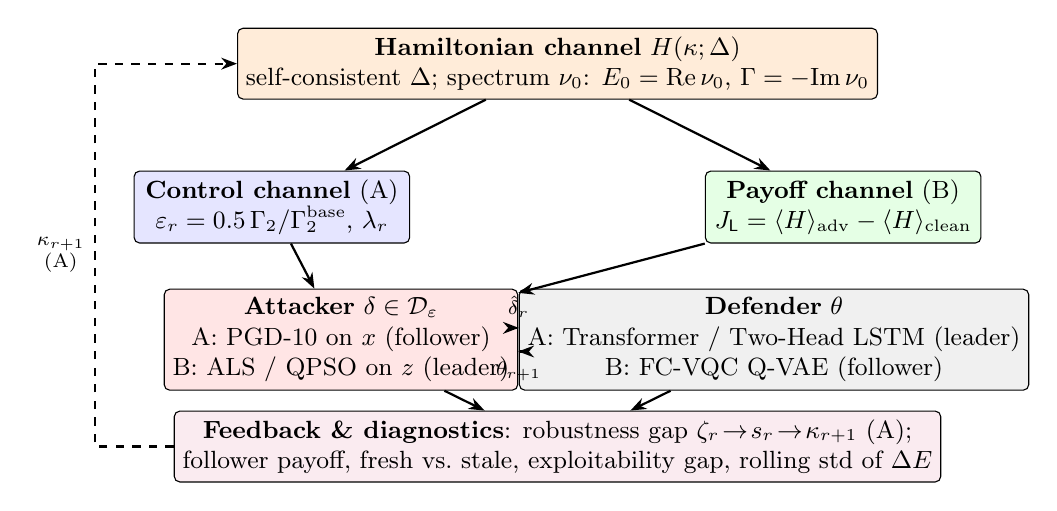
\begin{tikzpicture}[
  box/.style={draw, rounded corners=2pt, align=center, font=\small, minimum height=9mm, inner sep=3pt},
  arr/.style={-{Stealth[length=2mm]}, thick}]
\node[box, fill=orange!15, minimum width=7.6cm] (H) {\textbf{Hamiltonian channel} $H(\kappa;\Delta)$\\ self-consistent $\Delta$; spectrum $\nu_0$: $E_0=\mathrm{Re}\,\nu_0$, $\Gamma=-\mathrm{Im}\,\nu_0$};
\node[box, fill=blue!10, below left=9mm and -2.2cm of H, minimum width=3.5cm] (C) {\textbf{Control channel} (A)\\ $\varepsilon_r=0.5\,\Gamma_2/\Gamma_2^{\mathrm{base}}$, $\lambda_r$};
\node[box, fill=green!10, below right=9mm and -2.2cm of H, minimum width=3.5cm] (P) {\textbf{Payoff channel} (B)\\ $J_{\mathsf L}=\langle H\rangle_{\mathrm{adv}}-\langle H\rangle_{\mathrm{clean}}$};
\node[box, fill=red!10, below=24mm of H, xshift=-2.75cm, minimum width=3.4cm] (ATT) {\textbf{Attacker} $\delta\in\mathcal D_\varepsilon$\\ A: PGD-10 on $x$ (follower)\\ B: ALS / QPSO on $z$ (leader)};
\node[box, fill=gray!12, below=24mm of H, xshift=2.75cm, minimum width=3.4cm] (DEF) {\textbf{Defender} $\theta$\\ A: Transformer / Two-Head LSTM (leader)\\ B: FC-VQC Q-VAE (follower)};
\node[box, fill=purple!8, below=9mm of $(ATT)!0.5!(DEF)$, minimum width=7.6cm] (FB) {\textbf{Feedback \& diagnostics}: robustness gap $\zeta_r\!\to\! s_r\!\to\!\kappa_{r+1}$ (A);\\ follower payoff, fresh vs.\ stale, exploitability gap, rolling std of $\Delta E$};
\draw[arr] (H) -- (C); \draw[arr] (H) -- (P);
\draw[arr] (C) -- (ATT); \draw[arr] (P) -- (ATT);
\draw[arr] ([yshift=1.5mm]ATT.east) -- node[above, font=\scriptsize]{$\hat\delta_r$} ([yshift=1.5mm]DEF.west);
\draw[arr] ([yshift=-1.5mm]DEF.west) -- node[below, font=\scriptsize]{$\theta_{r+1}$} ([yshift=-1.5mm]ATT.east);
\draw[arr] (DEF) -- (FB); \draw[arr] (ATT) -- (FB);
\draw[arr, dashed] (FB.west) -- ++(-1.0,0) |- node[pos=0.25, left, font=\scriptsize, align=center]{$\kappa_{r+1}$\\(A)} (H.west);
\end{tikzpicture}}
\caption{The Hamiltonian--Stackelberg game loop. The same operator family enters as a control channel (Study~A: spectra set $\varepsilon$ and $\lambda$, a validation signal rescales the couplings) or as a payoff channel (Study~B: the leader maximises an energy shift). In both studies a perturbation is computed against the current defender, then the defender is updated against it.}
\label{fig:loop}
\end{figure}

\begin{table*}[t]
\centering
\caption{Instantiations of the building blocks: Study~A on classification (fraud detection) and regression (bond-yield forecasting), and Study~B}
\label{tab:inst}
\footnotesize
\setlength{\tabcolsep}{3pt}
\begin{tabular}{@{}>{\raggedright\arraybackslash}p{2.0cm}>{\raggedright\arraybackslash}p{4.9cm}>{\raggedright\arraybackslash}p{4.9cm}>{\raggedright\arraybackslash}p{4.9cm}@{}}
\toprule
Element & Study A, classification (fraud) & Study A, regression (bond yield) & Study B (quantum) \\
\midrule
Scenario & Fraudster alters own fraudulent transactions to evade a deployed detector (Sec.~\ref{sec:threatA}) & Adversary corrupts the market data in the forecaster's look-back window to move its next-day forecast (Sec.~\ref{sec:threatR}) & Adversary corrupts a Q-VAE's latent code to shift the energy of the decoded state (Sec.~\ref{sec:threatB}) \\
Leader & Defender (detector $f_\theta$) & Defender (forecaster $f_\theta$) & Attacker (latent $\delta z$) \\
Follower & Attacker (input $\delta$) & Attacker (window $\delta$) & Defender (FC-VQC $\theta$) \\
Attacker strategy space & $\mathcal D_{\varepsilon_r}$: $\|\delta_i\|_\infty\le\varepsilon_r$ on fraud rows, $\delta_i=0$ on legitimate rows; 18 features (30 in Sec.~\ref{sec:verA}) & $\mathcal D_{\varepsilon_r}$: $\|\delta_i\|_\infty\le\varepsilon_r$ on the 19 market features of a 10-day window, 0 on calendar and regime indicators, Eq.~\eqref{eq:DR} & $\mathcal D_\varepsilon\subset\mathbb R^q$, $\|\delta z\|_\infty\le\varepsilon=0.1$ \\
Defender strategy space & $\Theta=\mathbb R^{70{,}593}$ (detector weights; $\mathbb R^{71{,}361}$ in Sec.~\ref{sec:verA}) & $\Theta=\mathbb R^{12{,}258}$ (forecaster weights) & FC-VQC rotation angles ($3qK$ per block) \\
Attacker utility $u_{\mathrm{att}}$ & BCE of $f_\theta(x{+}\delta)$ on true label, Eq.~\eqref{eq:uatt} & Squared error of the forecast, Eq.~\eqref{eq:uattR} & Energy shift $J_{\mathsf L}$, Eq.~\eqref{eq:JL} \\
Defender utility $u_{\mathrm{def}}$ & $-[(1{-}\lambda_r)\cL+\lambda_r\cL_{\mathrm{adv}}]$, focal loss, Eq.~\eqref{eq:defobj} & $-[(1{-}\lambda_r)\cL_{\mathrm{TH}}+\lambda_r\cL_{\mathrm{TH,adv}}]$, two-head loss, Eq.~\eqref{eq:defobjR} & $-J_{\mathsf F}$, adversarial ELBO, Eq.~\eqref{eq:JF} \\
Payoff change per round & $\theta$ (every batch); $\varepsilon_r,\lambda_r$ from controller & $\theta$ (every batch); $\varepsilon_r,\lambda_r$ from controller & $\theta_r$ only; $H$, $\varepsilon$ fixed \\
Attacker best response & PGD, 10 steps, per batch (Alg.~\ref{alg:pgd}) & PGD, 10 steps, per batch, on market features (Alg.~\ref{alg:pgdR}) & Better of ALS and QPSO, per epoch (Algs.~\ref{alg:als}, \ref{alg:qpso}) \\
Defender best response & One AdamW step per batch (Alg.~\ref{alg:A}) & One AdamW step per batch (Alg.~\ref{alg:A}) & One parameter-shift step per epoch (Alg.~\ref{alg:ps}) \\
Test-time response & PGD ensemble and transfer (Alg.~\ref{alg:eval}) & PGD ensemble and transfer (Alg.~\ref{alg:evalR}) & ALS+QPSO on trained Q-VAE; MNIST: PGD-20 \\
Hamiltonian role & Control: $\Gamma(H_1),\Gamma(H_2)\to(\lambda_r,\varepsilon_r)$ & Control: $\Gamma(H_1),\Gamma(H_2)\to(\lambda_r,\varepsilon_r)$ & Payoff and data: ground states of $H_1,H_2,\HV$ \\
Spectrum & Complex, general eigensolver & Complex, general eigensolver & Real, Hermitian eigensolver \\
Feedback & Validation gap $\to$ couplings & Validation gap $\to$ couplings & None ($\Phi\equiv0$) \\
Diagnostics & (a)--(c) of Def.~\ref{def:diag} & (a)--(c) of Def.~\ref{def:diag} & (a), (d) of Def.~\ref{def:diag} \\
Quantum parts & None; all classical (Sec.~\ref{sec:hwA}) & None; all classical (Sec.~\ref{sec:regA}) & FC-VQC circuits, parameter-shift evaluations, $\langle H\rangle$ (Sec.~\ref{sec:qc}) \\
Hamiltonian solver & Alg.~\ref{alg:sc}, complex, CPU & Alg.~\ref{alg:sc}, complex, CPU & Alg.~\ref{alg:sc}, Hermitian, CPU \\
Hardware & CPU (GPU in Sec.~\ref{sec:verA}) & CPU & NVIDIA A6000 GPU \\
\bottomrule
\end{tabular}
\end{table*}

\begin{table}[t]
\centering
\caption{Notation shared by the studies}
\label{tab:notation}
\footnotesize
\setlength{\tabcolsep}{3pt}
\begin{tabular}{@{}>{\raggedright\arraybackslash}p{1.7cm}>{\raggedright\arraybackslash}p{6.6cm}@{}}
\toprule
Symbol & Meaning \\
\midrule
$\theta\in\Theta$ & defender's strategy: detector, forecaster or circuit parameters \\
$\delta\in\mathcal D_\varepsilon$ & attacker's strategy: perturbation of an input $x$ or latent code $z$, $\|\delta\|_\infty\le\varepsilon$ \\
$\mathsf L,\mathsf F$ & leader and follower \\
$u_{\mathrm{att}},u_{\mathrm{def}}$ & attacker's and defender's utilities (maximised) \\
$\BR_{\mathsf F}$ & follower's best-response set, Eq.~\eqref{eq:br} \\
$r$; $\varepsilon_r,\lambda_r$ & round; budget and weight of the adversarial loss term in round $r$ \\
$H(\kappa;\Delta)$ & Hamiltonian channel with couplings $\kappa$ and self-consistent order parameter $\Delta$ (or field $\phi$ for $\HV$) \\
$\nu_0,E_0,\Gamma$ & ground eigenvalue, its energy $\mathrm{Re}\,\nu_0$ and decay rate $-\mathrm{Im}\,\nu_0$ \\
$m$ & mixing fraction of the self-consistent iteration \\
$\zeta_r,s_r$ & relative robustness gap on validation and feedback signal, Eq.~\eqref{eq:feedback} \\
$w$ & per-feature PGD step weights from the spectra of $H_1,H_2$ \\
$\tau$ & error increase that breaks a forecast (regression) \\
$J_{\mathsf L},J_{\mathsf F},\Delta E$ & leader's energy shift, follower's adversarial ELBO, realised energy gain (Study~B) \\
\bottomrule
\end{tabular}
\end{table}

%=====================================================================
\section{The Hamiltonian Layer}\label{sec:ham}
%=====================================================================
This section derives the three operators shared by both studies, gives the spectrum of the two-mode operators in closed form (Theorem~\ref{thm:spec}), shows that their self-consistent iterations converge (Theorem~\ref{thm:sc}, Section~\ref{sec:conv}), gives the qubit representations used in Study~B, and describes how the operators are solved on CPU and GPU (Section~\ref{sec:cpugpu}). Throughout, $\omega_k$ denote level energies (not to be confused with the attack budget $\varepsilon$), $\Delta_j$ self-consistent transition fields, and a tilde marks an operator on the auxiliary space of thermofield dynamics.

\subsection{Thermofield dynamics of open systems}\label{sec:tfd}
The operators describe dissipative atomic systems, whose density operator $\rho$ obeys a master equation $\dot\rho=\frac{1}{i\hbar}[H,\rho]+\Lambda[\rho]$ with Hamiltonian part $H$ and dissipator $\Lambda$~\cite{lindblad1976}. To treat it with Schr\"odinger-equation methods we use thermofield dynamics (TFD)~\cite{takahashi1975,patel2026,patel2025}: the density operator is represented as a state vector $|\rho(t)\rangle=\rho(t)|I\rangle$ in an enlarged space $\mathcal H\otimes\widetilde{\mathcal H}$, where $|I\rangle$ is the identity state and the tilde operators act on an auxiliary copy of the original space. Original and tilde operators are related by the TFD identities
\begin{equation}
A|I\rangle=\widetilde A^{\dagger}|I\rangle,\qquad A^{\dagger}|I\rangle=\widetilde A|I\rangle,
\label{eq:tfdid}
\end{equation}
for each mode operator $A$. With \eqref{eq:tfdid} the master equation takes the Schr\"odinger-like form
\begin{equation}
\partial_t|\rho(t)\rangle=-i\widehat H\,|\rho(t)\rangle,
\label{eq:tfd}
\end{equation}
where the generator $\widehat H$ contains original, tilde and dissipative contributions. Because of the dissipator, $\widehat H$ is non-Hermitian: energy terms enter through $1/(i\hbar)$ and damping rates $\gamma$ with real coefficients~\cite{ashida2020}.

\subsection{Two-mode operators \texorpdfstring{$H_1$ and $H_2$}{H1 and H2}}\label{sec:h12}
$H_1$ and $H_2$ follow the soliton-pair model of a three-level atom in which two optical fields drive the transitions from a common level $|0\rangle$ to levels $|1\rangle$ and $|2\rangle$~\cite{eleuch2003}. There is no direct transition between $|1\rangle$ and $|2\rangle$, so the two transitions are treated separately and the atomic Hamiltonian is
\begin{equation}
H_{\mathrm{at}}=H_{\mathrm{lev}}+V_{01}+V_{02},
\label{eq:Hat}
\end{equation}
where $H_{\mathrm{lev}}$ contains the atomic level energies and $V_{01}$, $V_{02}$ the two field-induced transitions, each with its own coupling strength and damping rate. In TFD form \eqref{eq:tfd} the generator splits by transition, $\widehat H=\widehat H_1+\widehat H_2$, and each $\widehat H_j$ acts on both the original and the auxiliary space.

Each $\widehat H_j$ contains products of several creation and annihilation operators, which make the evolution hard to solve directly. The Hartree--Fock approximation replaces these products by expectation values times lower-order operator products. For the transition involving modes $a$ and $b$ it introduces the transition field
\begin{equation}
\Delta_1=\langle a^\dagger b\rangle=\langle b^\dagger a\rangle=\langle \tilde a^\dagger\tilde b\rangle=\langle \tilde b^\dagger\tilde a\rangle,
\label{eq:Delta1}
\end{equation}
the mean transition coherence between the two modes, determined self-consistently. After the approximation the generator separates into original and auxiliary parts, $\widehat H_1=H_1-\widetilde H_1$, and the original-space part is bilinear in the mode operators. The second transition connects $|0\rangle$ to $|2\rangle$ and follows the same procedure with mode $c$, field $\cE_2$, coupling $g_2$, damping $\gamma_2$ and transition field
\begin{equation}
\Delta_2=\langle a^\dagger c\rangle=\langle c^\dagger a\rangle=\langle \tilde a^\dagger\tilde c\rangle=\langle \tilde c^\dagger\tilde a\rangle .
\label{eq:Delta2}
\end{equation}

With modes truncated to one excitation ($n_{\max}=1$), both reduced operators act on $\mathbb C^4$ and share the form
\begin{align}
H(\omega_a,\omega_b,\gamma,g,\cE;\Delta)&=c_a n_a+c_b n_b+c_{ab}\,(a\ad b+b\ad a),\label{eq:H2mode}\\
c_a=\frac{\omega_a}{2i\hbar}+\frac{\gamma}{2},\quad c_b&=\frac{\omega_b}{i\hbar}-\frac{\gamma}{2},\quad c_{ab}=\frac{g\cE}{i\hbar}-\gamma\Delta,\nonumber
\end{align}
with level energies $\omega$, damping $\gamma$, coupling $g$ and drive amplitude $\cE$~\cite{eleuch2003}: $H_1=H(\omega_0,\omega_1,\gamma_1,g_1,\cE_1;\Delta_1)$ couples modes $a$ and $b$, and $H_2=H(\omega_0,\omega_2,\gamma_2,g_2,\cE_2;\Delta_2)$ couples $a$ and $c$. The first two terms are the single-mode contributions with their damping corrections; the last couples the modes through the optical field and the Hartree--Fock transition field. The nonlinear problem is thus reduced to two-mode operators whose coefficients depend on the system parameters and on $\Delta_j$.

In the released solver, which produced every result in this paper, the fixed-point iteration of Definition~\ref{def:hc} ($m=0.3$) evaluates $\hat O_1=ab$ and $\hat O_2=ac$ rather than the coherences $a^\dagger b$ and $a^\dagger c$ of \eqref{eq:Delta1}--\eqref{eq:Delta2}. The ground state of \eqref{eq:H2mode} lies in the single-excitation subspace, where $\langle ab\rangle$ and $\langle ac\rangle$ vanish identically, so the iteration converges to $\Delta_j=0$ and $H_1$, $H_2$ reduce to their drive-only form. Iterating the real parts of $\langle a^\dagger b\rangle$ and $\langle a^\dagger c\rangle$ instead converges to a different fixed point, $\Delta_{1,2}=0.441$, and shifts $E_0$ from $-0.01371$ to $-0.05791$. The quantities that enter the experiments change little: the decay rate at the base parameters moves from 0.16618 to 0.17266 (3.9\%), the controller's budget range from $[0.3461,0.6586]$ to $[0.3686,0.6428]$ (final budget 2.4\% lower), the maximum attack step weight from 1.488 to 1.432, and Study~B's targets by less than $10^{-3}$ in fidelity.

The reduced operators can be diagonalised in closed form, which makes their ground state, energy and decay rate explicit functions of the parameters.

\begin{theorem}[Closed-form spectrum of $H_1$ and $H_2$]\label{thm:spec}
Let $\hbar=1$, $\omega_a,\omega_b,g,\cE\ge0$, $\gamma>0$ and $\Delta\ge0$ in \eqref{eq:H2mode}, and write $\mu=(c_a+c_b)/2=-i(\omega_a+2\omega_b)/4$, $d=(c_a-c_b)/2=\gamma/2+i(\omega_b-\omega_a/2)/2$, $w=d^2+c_{ab}^2$ and $s=\sqrt w$ for the principal square root. Then:
\begin{enumerate}
\item[(i)] the spectrum of $H$ is $\{0,\ c_a+c_b,\ \mu+s,\ \mu-s\}$;
\item[(ii)] if $\mathrm{Im}\,w>0$, the ground eigenvalue (smallest real part) is $\nu_0=\mu-s$; it is simple, its eigenvector lies in $\mathrm{span}\{|10\rangle,|01\rangle\}$, and
\begin{equation}
E_0=-\sqrt{\tfrac{|w|+\mathrm{Re}\,w}{2}},\qquad \Gamma=\tfrac{\omega_a+2\omega_b}{4}+\sqrt{\tfrac{|w|-\mathrm{Re}\,w}{2}};
\label{eq:gammaclosed}
\end{equation}
\item[(iii)] if $b:=\gamma(\omega_b-\omega_a/2)/2>0$, then $\mathrm{Im}\,w>0$ for every $\Delta\ge0$; and at $\Delta=0$, where $w=d^2-g^2\cE^2$, the decay rate is strictly increasing in the coupling $g$, with
\begin{equation}
0<\frac{d\Gamma}{dg}=\frac{g\cE^2\,\mathrm{Im}\,s}{|s|^2}\le\frac{g\cE^2}{\sqrt b}\qquad(g>0).
\label{eq:dgamma}
\end{equation}
\end{enumerate}
\end{theorem}

\begin{proof}
(i) The number operator $n_a+n_b$ commutes with $n_a$, $n_b$ and $a\ad b+b\ad a$, so in the basis $\{|00\rangle,|01\rangle,|10\rangle,|11\rangle\}$ the operator \eqref{eq:H2mode} is block diagonal: it acts as $0$ on $|00\rangle$, as $c_a+c_b$ on $|11\rangle$, and as $\begin{pmatrix}c_a&c_{ab}\\c_{ab}&c_b\end{pmatrix}$ on $\{|10\rangle,|01\rangle\}$, whose characteristic polynomial $(\nu-\mu)^2-d^2-c_{ab}^2$ has roots $\mu\pm s$.
(ii) The principal root has $\mathrm{Re}\,s\ge0$, and $\mathrm{Re}\,s=0$ would make $w=s^2=-(\mathrm{Im}\,s)^2$ real, so $\mathrm{Im}\,w>0$ forces $\mathrm{Re}\,s>0$. Since $\mathrm{Re}\,\mu=\mathrm{Re}(c_a+c_b)=0$, the real parts of the four eigenvalues are $0,0,+\mathrm{Re}\,s,-\mathrm{Re}\,s$, so $\mu-s$ is the unique eigenvalue of smallest real part and belongs to the one-excitation block. With $\mathrm{Re}\,s=\sqrt{(|w|+\mathrm{Re}\,w)/2}$ and $\mathrm{Im}\,s=\sqrt{(|w|-\mathrm{Re}\,w)/2}$ for $\mathrm{Im}\,w>0$, $E_0=\mathrm{Re}\,\nu_0=-\mathrm{Re}\,s$ and $\Gamma=-\mathrm{Im}\,\nu_0=(\omega_a+2\omega_b)/4+\mathrm{Im}\,s$.
(iii) With $c_{ab}=-ig\cE-\gamma\Delta$, $c_{ab}^2=-g^2\cE^2+\gamma^2\Delta^2+2i\gamma\Delta g\cE$ and $\mathrm{Im}\,d^2=2\,\mathrm{Re}\,d\,\mathrm{Im}\,d=b$, so $\mathrm{Im}\,w=b+2\gamma\Delta g\cE\ge b>0$. At $\Delta=0$, differentiating $s^2=d^2-g^2\cE^2$ gives $ds/dg=-g\cE^2/s$, hence $d\Gamma/dg=\mathrm{Im}(ds/dg)=-g\cE^2\,\mathrm{Im}(1/s)=g\cE^2\,\mathrm{Im}\,s/|s|^2$, which is positive because $\mathrm{Im}\,s>0$, and at most $g\cE^2/|s|\le g\cE^2/\sqrt b$ because $|s|^2=|w|\ge\mathrm{Im}\,w=b$.
\end{proof}

At the Study~A parameters, $\hbar=1$, $\omega_0=\omega_1=\omega_2=\gamma_{1,2}=g_{1,2}=0.1$ and $\cE_{1,2}=1$, $H_1$ and $H_2$ have identical coefficients and therefore identical spectra. Here $b=0.0025>0$, and Theorem~\ref{thm:spec} gives $\{-0.01371-0.16618i,\ 0,\ -0.15000i,\ +0.01371+0.01618i\}$, with $E_0=-0.01371$ and $\Gamma=0.16618$. An independent implementation (\texttt{numpy.linalg.eig}) reproduces the closed form to within $4{\times}10^{-16}$ for every coupling $g\in[0,0.3]$.

\subsection{Spectral treatments in the two studies}\label{sec:spec}
Both studies build $H_1$, $H_2$ and $\HV$ from the same reference solver with the same parameters (Table~\ref{tab:hamcheck}); they differ only in how the spectrum is read. Study~A uses a general eigensolver (\texttt{numpy.linalg.eig}) and the full complex spectrum, because the operators are non-Hermitian and the control channel needs the decay rate $\Gamma=-\mathrm{Im}\,\nu_0$. Study~B obtains its target ground states with a Hermitian eigensolver (\texttt{numpy.linalg.eigh}), applied to $H_1$ directly and to the entrywise real parts of $H_2$ and $\HV$, as in the reference solver; the resulting energies are real. Re-running the reference solver reproduces Study~B's ground energies (Table~\ref{tab:sc}: $-0.1118$ and $-0.0500$ exactly; $-2.0005$ against $-2.0004$ for $\HV$), which confirms this treatment. For a non-Hermitian matrix a Hermitian eigensolver reads only one triangle and the real diagonal, so it diagonalises a different matrix without warning; Study~B's targets are therefore ground states of these Hermitian surrogates, not of the non-Hermitian operators whose decay rates drive Study~A. We keep each study's treatment as run and report them side by side.

\begin{table}[t]
\centering
\caption{The shared operators under both spectral treatments (base parameters). Complex: lowest-real-part eigenvalue $\nu_0$ from \texttt{eig} (Study~A). Hermitian: lowest eigenvalue from \texttt{eigh} as in the reference solver (Study~B). Parameters: $H_1,H_2$: $\omega_{0,1,2}{=}\gamma{=}g{=}0.1$, $\cE{=}1$; $\HV$: $\omega_{0,1}{=}1$, $g_1{=}0.15$, $h{=}1$, $\cE_1{=}0.5{+}0.3i$, $\gamma_1{=}0.1$, $\eta_T{=}1$. Rows A and B recomputed from the reference solver; last row as listed in Table~\ref{tab:sc}.}
\label{tab:hamcheck}
\footnotesize
\setlength{\tabcolsep}{2.5pt}
\resizebox{\columnwidth}{!}{\begin{tabular}{lccc}
\toprule
& $H_1$ & $H_2$ & $\HV$\\
\midrule
Complex $\nu_0$ (A) & $-0.01371-0.16618i$ & $-0.01371-0.16618i$ & $-1.99943-0.14996i$\\
Order/field (A) & $\approx0$ & $\approx0$ & $\phi=0.00601$\\
Hermitian $E_0$ (B) & $-0.1118$ & $-0.0500$ & $-2.0005$\\
Table~\ref{tab:sc} & $-0.1118$ & $-0.0500$ & $-2.0004$\\
\bottomrule
\end{tabular}}
\end{table}

\subsection{Four-qubit operator \texorpdfstring{$\HV$}{HV}}\label{sec:hv}
$\HV$ describes a two-level atom interacting with an external electric field and a magnetic field~\cite{patel2026,patel2025}. With fermionic creation and annihilation operators $a^\dagger,a$ and $b^\dagger,b$ for the two levels, the rotating-wave Hamiltonian is
\begin{equation}
\begin{aligned}
H&=\omega_0 a^\dagger a+\omega_1 b^\dagger b+i g_1\hbar\big(a^\dagger b\,\cE_1+b^\dagger a\,\cE_1^{*}\big)+M,\\
M&=\begin{pmatrix}f_{00}\,\mathcal B&0\\0&f_{11}\,\mathcal B\end{pmatrix},
\end{aligned}
\label{eq:Hfermi}
\end{equation}
where $\omega_0,\omega_1$ are the level energies, $g_1$ the field coupling, $\cE_1$ the applied field and $M$ the magnetic interaction with field $\mathcal B$ and coupling strengths $f_{00}$, $f_{11}$ of the excited and ground levels. The operators obey $\{a_i,a_j^\dagger\}=\delta_{ij}$ and $\{a_i,a_j\}=\{a_i^\dagger,a_j^\dagger\}=0$. The first two terms of \eqref{eq:Hfermi} are the level energies, the next two the field-driven transitions in both directions, and $M$ the magnetic contribution. Coupling to a thermal environment adds the dissipator
\begin{equation}
\begin{aligned}
\Lambda[\rho]={}&\tfrac{\gamma_1}{2}(1+\eta_T)\big([b^\dagger a,\,a^\dagger b\rho]+[b^\dagger a\rho,\,a^\dagger b]\big)\\
&+\tfrac{\gamma_1}{2}\,\eta_T\big([a^\dagger b,\,\rho\, b^\dagger a]+[a^\dagger b\rho,\,b^\dagger a]\big),
\end{aligned}
\label{eq:dissT}
\end{equation}
with damping rate $\gamma_1$ and thermal occupation factor $\eta_T$; the two terms describe the dissipative processes associated with the thermal environment.

Applying the TFD identities \eqref{eq:tfdid} to $a$, $b$ and their tilde copies turns the master equation into the form \eqref{eq:tfd}, whose generator contains the original Hamiltonian, its tilde counterpart and the terms generated by $\Lambda$; unlike the Hamiltonian of a closed system it therefore includes environmental damping. The generator contains products of several fermionic operators acting on both spaces. To represent it on qubits, each fermionic operator is mapped to Pauli operators with the Bravyi--Kitaev transformation~\cite{bravyi2002}, which preserves the anticommutation relations:
\begin{equation}
a_j^{(\dagger)}=\tfrac12\big(X_{\mathcal U(j)}X_jZ_{\mathcal P(j)}\mp iX_{\mathcal U(j)}Y_jZ_{\mathcal R(j)}\big),
\label{eq:bk}
\end{equation}
with the upper sign for $a_j^\dagger$ and the lower for $a_j$. Here $X_j,Y_j,Z_j\equiv\sigma^x_j,\sigma^y_j,\sigma^z_j$ act on qubit $j$, and $\mathcal U(j)$, $\mathcal P(j)$, $\mathcal R(j)$ are the update, parity and remainder sets of mode $j$; a subscript set denotes the product over its qubits. The two original and two tilde modes are encoded in a four-qubit register, $\dim=2^4=16$.

Substituting \eqref{eq:bk} gives a sum of Pauli strings on the four qubits, which group into energy, field-coupling and dissipative contributions. The operator used throughout this paper is the one implemented in the released solver,
\begin{align}
\HV&=H_{\mathrm{energy}}+H_{\mathrm{coupling}}(\phi)+\tfrac{\gamma_1}{16}\big(\eta_T D_\eta+D_0\big),\label{eq:HV}\\
H_{\mathrm{energy}}&=-\tfrac{\omega_0}{2}(\sigma^z_0-\sigma^z_2)-\tfrac{\omega_1}{2}(\sigma^z_1\sigma^z_0+\sigma^z_3\sigma^z_2\sigma^z_1),\nonumber\\
H_{\mathrm{coupling}}(\phi)&=\tfrac{i g_1 h\phi}{4}\big(C\,\cE_1+C'\,\cE_1^{*}\big),\nonumber
\end{align}
where the field coupling depends on a self-consistent field $\phi$ and the dissipative part on two fixed Pauli sums, $D_\eta$ (multiplied by $\eta_T$) and $D_0$. The Pauli sums $C$, $C'$, $D_\eta$ and $D_0$ are listed term by term in Appendix~\ref{app:hv}; the listing was generated from the solver and verified by rebuilding the full $16{\times}16$ matrix from it. The magnetic terms of \eqref{eq:Hfermi} ($\mathcal B$, $f_{00}$, $f_{11}$) are not included in this operator. The field is iterated as $\phi_{n+1}=0.5\sqrt{\langle\sigma^x_0\rangle^2+\langle\sigma^y_0\rangle^2}+0.5\,\phi_n$. At the Study~A parameters ($\omega_0=\omega_1=1$, $g_1=0.15$, $h=1$, $\cE_1=0.5+0.3i$, $\gamma_1=0.1$, $\eta_T=1$) it converges to $\phi=0.00601$. $\HV$ is the third benchmark system of Study~B and is computed and logged, but not used for control, in Study~A.

\subsection{Convergence of the self-consistent iterations}\label{sec:conv}
Each operator is solved by the fixed-point iteration of Definition~\ref{def:hc}, $x_{n+1}=F(x_n)$, implemented by Algorithm~\ref{alg:sc}. For $\HV$ the variable is the field, $F(\phi)=\tfrac12\sqrt{\langle\sigma^x_0\rangle^2+\langle\sigma^y_0\rangle^2}+\tfrac12\phi$, with the expectation values taken in the ground state of $\HV(\phi)$. We test convergence under both spectral treatments, at the three coupling scales the controller visits ($\eta_T$ multiplied by $1-0.5s$ for $s\in\{+1,0,-1\}$), and from four initial values $\phi_0\in\{10^{-4},0.1,0.5,1\}$, iterating until $|\phi_{n+1}-\phi_n|<10^{-10}$ (Table~\ref{tab:conv}, Fig.~\ref{fig:conv_hv}). The following result says when such an iteration converges, how fast, and to which point.

\begin{theorem}[Convergence of the self-consistent iteration]\label{thm:sc}
Let $I\subset\mathbb R$ be a closed interval, $G:I\to\mathbb R$ an $L$-Lipschitz map, $m\in(0,1]$, and $T(x)=m\,G(x)+(1-m)\,x$, the update of Definition~\ref{def:hc}. If $T(I)\subseteq I$ and $\rho:=(1-m)+mL<1$, then $T$ has a unique fixed point $x^\star\in I$, and for every $x_0\in I$ the iterates $x_{n+1}=T(x_n)$ satisfy $|x_n-x^\star|\le\rho^n|x_0-x^\star|$. If $G$ is differentiable at $x^\star$, the asymptotic contraction factor is $|1-m+m\,G'(x^\star)|$. If $G\equiv0$ on $I$, then $x^\star=0$ and $x_n=(1-m)^nx_0$ exactly.
\end{theorem}

\begin{proof}
For $x,y\in I$, $|T(x)-T(y)|\le(1-m)|x-y|+m|G(x)-G(y)|\le\rho|x-y|$, so $T$ is a contraction of the complete metric space $I$ into itself, and Banach's fixed-point theorem gives the unique fixed point and the geometric bound. Near $x^\star$, $T(x)-x^\star=T'(x^\star)(x-x^\star)+o(|x-x^\star|)$ with $T'(x^\star)=1-m+mG'(x^\star)$, which gives the asymptotic factor. If $G\equiv0$, $T(x)=(1-m)x$.
\end{proof}

For $H_1$ and $H_2$ the observable of the implemented iteration is $G(\Delta)=\mathrm{Re}\langle\psi_0(\Delta)|\hat O_j|\psi_0(\Delta)\rangle$ with $\hat O_1=ab$, $\hat O_2=ac$ and $m=0.3$. By Theorem~\ref{thm:spec}(ii)--(iii) the ground state lies in the one-excitation subspace for every $\Delta\ge0$, and $ab$ and $ac$ annihilate that subspace, so $G\equiv0$ on $I=[0,\Delta_0]$, which $T(\Delta)=0.7\Delta$ maps into itself. Theorem~\ref{thm:sc} then gives $\Delta_n=0.7^n\Delta_0\to0$, and the stopping rule $|\Delta_{n+1}-\Delta_n|=0.3\cdot0.7^n\Delta_0<10^{-8}$ first holds at $n=42$, i.e., in the 43rd iteration from $\Delta_0=0.1$. For $\HV$, $G(\phi)=\sqrt{\langle\sigma^x_0\rangle^2+\langle\sigma^y_0\rangle^2}$ and $m=0.5$. For a normalised state the Bloch vector of qubit 0 has length at most 1, so $G$ maps into $[0,1]$ and $T$ maps $I=[0,1]$ into itself; Theorem~\ref{thm:sc} applies whenever the Lipschitz constant of $G$ on $I$ is below 1, and then predicts an asymptotic factor $0.5+0.5\,G'(\phi^\star)$. We do not have an analytic bound on $G'$; the measurements below determine it.

The $\HV$ iteration converges in all 24 runs, in 25--34 iterations, and the four initial values reach the same fixed point $\phi^\star$ to within $2{\times}10^{-10}$, so the fixed point does not depend on the starting value over four orders of magnitude. At the fixed point the residual $|F(\phi^\star)-\phi^\star|$ is below $5{\times}10^{-11}$. The error contracts by a factor $|\phi_{n+1}-\phi^\star|/|\phi_n-\phi^\star|$ of 0.4995--0.4997 per iteration under the complex treatment and 0.5000 under the Hermitian treatment (Fig.~\ref{fig:conv_hv}b). By Theorem~\ref{thm:sc} this factor is $0.5+0.5\,G'(\phi^\star)$, so the measured factors put the slope of the expectation term below $10^{-3}$ in magnitude at the fixed points: the ground-state coherence depends only weakly on $\phi$, and the iteration converges geometrically, halving the error at every step. The fixed points increase monotonically with the coupling scale, from $\phi^\star=0.00306$ to $0.00883$ (complex), and reproduce the $\phi$ column of Table~\ref{tab:ctrl}.

$H_1$ and $H_2$ converge exactly as Theorem~\ref{thm:sc} predicts: the iteration contracts by 0.7 per step from any starting value and converges to $\Delta_j=0$, and the solver stops after 43 iterations from $\Delta_0=0.1$.

\begin{figure*}[t]
\centering
\includegraphics[width=0.85\textwidth]{figs/hv_convergence.pdf}
\caption{Convergence of the $\HV$ field iteration (complex treatment, $\phi_0=0.1$) at the three coupling scales of the controller. (a) Iterates $\phi_n$. (b) Distance to the fixed point on a log scale; the dash-dotted line is $0.1\cdot2^{-n}$, the rate implied by the mixing weight $m=0.5$. Values are listed in Table~\ref{tab:conv}.}
\label{fig:conv_hv}
\end{figure*}

\begin{table}[t]
\centering
\caption{Convergence of the $\HV$ field iteration from $\phi_0\in\{10^{-4},0.1,0.5,1\}$ (tolerance $10^{-10}$). Spread: largest difference between the fixed points reached from the four starts. Contraction: median of $|\phi_{n+1}-\phi^\star|/|\phi_n-\phi^\star|$ over the tail.}
\label{tab:conv}
\footnotesize
\setlength{\tabcolsep}{3pt}
\begin{tabular}{lrcccc}
\toprule
Treatment & $s$ & $\phi^\star$ & Spread & Iterations & Contraction\\
\midrule
Complex & $+1$ & 0.003063 & $1.8{\times}10^{-10}$ & 25--34 & 0.4997\\
 & $0$ & 0.006010 & $1.7{\times}10^{-10}$ & 26--34 & 0.4996\\
 & $-1$ & 0.008825 & $1.5{\times}10^{-10}$ & 27--34 & 0.4995\\
Hermitian & $+1$ & 0.003037 & $1.8{\times}10^{-10}$ & 25--34 & 0.5000\\
 & $0$ & 0.006092 & $1.8{\times}10^{-10}$ & 26--34 & 0.5000\\
 & $-1$ & 0.009162 & $1.5{\times}10^{-10}$ & 27--34 & 0.5000\\
\bottomrule
\end{tabular}
\end{table}

\subsection{Qubit mapping of \texorpdfstring{$H_1$ and $H_2$}{H1 and H2}}\label{sec:qmap}
For a circuit, the bosonic operators of $H_1$ and $H_2$ are mapped to qubits. With $n_{\max}=1$ the modes are hard-core bosons, and for mode $j$ of $n$,
\begin{equation}
a_j\ad=\tfrac12(X_j-iY_j)\otimes\textstyle\bigotimes_{k\ne j}I_k .
\label{eq:jw}
\end{equation}
Because the modes are spatially separated bosons that commute, no Jordan--Wigner parity string is needed; this differs from the fermionic modes of $\HV$, which require the Bravyi--Kitaev mapping \eqref{eq:bk}. Study~B verified $\|H_{\mathrm{mapped}}-H_{\mathrm{direct}}\|_F=0$ to machine precision for $H_1$ and $H_2$.

\subsection{Solving the Hamiltonians on CPU and GPU}\label{sec:cpugpu}
Every operator is affine in its coupling and in its self-consistent variable: $H_j(g_j,\Delta_j)=B^{(j)}_0+g_jB^{(j)}_g+\Delta_jB^{(j)}_\Delta$ for $j=1,2$, and $\HV(\phi,\eta_T)=A_0+\phi A_\phi+\eta_TA_\eta$. The component matrices are obtained from the reference solver by evaluating it at unit and zero arguments, and the decomposition is exact (checked to $10^{-13}$ at independent argument values). One iteration of Algorithm~\ref{alg:sc} therefore costs one matrix assembly, one eigendecomposition of a $4{\times}4$ or $16{\times}16$ complex matrix, $O(d^3)$ with $d\le16$, and one expectation value.

On the CPU path, used for all reported results, the reference implementation solves one operator at a time in NumPy: \texttt{numpy.linalg.eig} (LAPACK, general complex matrices) for the complex treatment and \texttt{numpy.linalg.eigh} for the Hermitian treatment, in double precision. In Study~A each controller round solves $H_1$, $H_2$ and $\HV$ once (Algorithm~\ref{alg:ctrl}); in Study~B the target ground states are solved once, before training.

On the GPU path the same iteration is written in PyTorch with \texttt{complex128} tensors and runs unchanged on a CPU or a CUDA device. A batch of $B$ coupling values is solved at once: the batched operators $(B,d,d)$ are assembled from the affine form, decomposed with \texttt{torch.linalg.eig} or \texttt{torch.linalg.eigh}, which accept batches of matrices, and the ground state of every batch element is selected with an index gather. Only the convergence test moves a scalar from the device to the host, once per iteration, and the loop stops when all $B$ elements have converged. On a CUDA device both eigensolvers synchronise the device with the host on every call, so the benefit of the GPU path lies in solving many operators or coupling values per call rather than in a single small solve.

Run on the CPU over the five coupling scales of Table~\ref{tab:ctrl}, the PyTorch implementation reproduces the reference ground-state eigenvalues of $H_1$, $H_2$ and $\HV$ to within $8{\times}10^{-15}$ and the field $\phi$ to within $5{\times}10^{-17}$; under the Hermitian treatment it reproduces the reference ground energies ($-0.1118$, $-0.0500$, $-2.0005$) exactly. Table~\ref{tab:solvetime} gives single-thread CPU timings on an Intel Xeon (2.10 GHz). One controller round costs 52.9 ms with NumPy and 34.4 ms with PyTorch; solving 1,000 coupling settings takes 54.6 s one at a time with NumPy and 4.36 s as one PyTorch batch, a factor of 12.5. GPU timings were not measured.

\begin{algorithm}[t]
\caption{Batched self-consistent solve of $H_1$, $H_2$ or $\HV$ (CPU or GPU)}\label{alg:sc}
\small
\begin{algorithmic}[1]
\Require components $(A_0,A_1,A_2)$ with $H(\kappa,x)=A_0+\kappa A_1+x A_2$; couplings $\kappa_1,\dots,\kappa_B$; update map $\Phi$; mixing $m$; tolerance $\tau$; treatment; device
\State $x_b\gets x_0$ for $b=1,\dots,B$ \Comment{tensors on the chosen device}
\Repeat
  \State $H_b\gets A_0+\kappa_bA_1+x_bA_2$ for all $b$ \Comment{one batched assembly}
  \If{complex treatment}
    \State $(\nu,V)\gets\mathrm{eig}(H_b)$; $k_b\gets\arg\min_k\mathrm{Re}\,\nu_{b,k}$; $\psi_b\gets V_{b,:,k_b}/\|V_{b,:,k_b}\|$
  \Else
    \State $(\nu,V)\gets\mathrm{eigh}(\bar H_b)$ with $\bar H_b=H_b$ ($H_1$) or $\mathrm{Re}\,H_b$ ($H_2$, $\HV$); $\psi_b\gets V_{b,:,1}$
  \EndIf
  \State $x'_b\gets m\,\Phi(\psi_b)+(1-m)\,x_b$ \Comment{$\Phi=\mathrm{Re}\langle\psi|\hat O_j|\psi\rangle$ or $\sqrt{\langle\sigma^x_0\rangle^2+\langle\sigma^y_0\rangle^2}$}
  \State $\mathrm{done}\gets\max_b|x'_b-x_b|<\tau$; $x\gets x'$ \Comment{one device--host transfer}
\Until{done}
\State \Return ground eigenvalues $\nu_{0,b}$, fixed points $x_b$, ground states $\psi_b$
\end{algorithmic}
\end{algorithm}

\begin{table}[t]
\centering
\caption{Hamiltonian solve times on CPU (one thread, Intel Xeon 2.10 GHz; median of repeated runs). NumPy: reference solver, one coupling value at a time. PyTorch: Algorithm~\ref{alg:sc} with all coupling values in one batch. Each entry solves $H_1$, $H_2$ and $\HV$ for every coupling value.}
\label{tab:solvetime}
\footnotesize
\begin{tabular}{rrrr}
\toprule
Coupling values & NumPy (ms) & PyTorch (ms) & Ratio\\
\midrule
1 & 52.9 & 34.4 & 1.5\\
5 & 267.5 & 62.0 & 4.3\\
100 & 5{,}160 & 475 & 10.9\\
1{,}000 & 54{,}575 & 4{,}363 & 12.5\\
\bottomrule
\end{tabular}
\end{table}

%=====================================================================
\section{Study A: Hamiltonian-Controlled Adversarial Training}\label{sec:studyA}
%=====================================================================
\subsection{Fraud data and leakage audit}\label{sec:dataA}
Study~A is run first on fraud detection, a classification task, and then, unchanged, on bond-yield forecasting, a regression task (Section~\ref{sec:regA}). The fraud dataset is synthetically generated and comprises 26,393 UPI and banking transactions: 21,848 legitimate (82.8\%) and 4,545 fraudulent (17.2\%), split 70/15/15 (18,475/3,959/3,959) with label stratification; StandardScaler normalisation is fit on the training split only. We have not validated how closely its distributions reflect real UPI fraud. Many raw columns encode the label: binary flags that are always 0 for legitimate transactions (e.g., \texttt{unusual\_device\_flag}), continuous features without class overlap (\texttt{receiver\_account\_age} is always 0 for fraud), and categories that map to a single class (\texttt{handle\_verification\_status}). Removing identifiers, timestamps, free text and label-encoding features reduces 64 raw signals to 14; four label-free composites (log amount, a keystroke typing-anomaly ratio, an amount-to-history ratio and a session engagement ratio) give 18 continuous features. After the audit every feature varies within both classes; the maximum single-feature training area under the ROC curve (AUC) is 0.948 (receiver transaction history) and the mean 0.650. Section~\ref{sec:verA} repeats the study on a public dataset of real card transactions.

Some leakage remains in the support of the features. The generator draws many fraud features from wider distributions than legitimate ones, so fraud values can lie outside the whole legitimate range (64\% of fraud values of \texttt{request\_amount\_roundness}, whose single-feature AUC is only 0.50). A rule with no learned parameters, which flags a transaction if any feature leaves the legitimate training range, reaches 0.995 precision and 0.836 recall with 3 false positives; logistic regression reaches a test AUC of 0.989. The task is nearly separable on clean data; we report this as a property of the benchmark.

\subsection{Detector}\label{sec:detA}
FraudTransformer embeds each of the 18 features as a token with a shared linear map $\mathbb R\to\mathbb R^{64}$, adds learned positional embeddings and a CLS token (sequence length 19), and applies two Transformer blocks~\cite{vaswani2017} (4 heads, $d_k{=}16$, FFN 64$\to$128$\to$64 with GELU, LayerNorm, dropout 0.4) and an MLP head (64$\to$32$\to$1); 70,593 parameters. Class imbalance is handled by focal loss~\cite{lin2017focal} ($\gamma_{\mathrm f}{=}2.0$, $\alpha_{\mathrm f}{=}0.75$). The baseline is trained with AdamW ($3{\times}10^{-4}$, weight decay $10^{-2}$), cosine decay ($T_{\max}{=}60$, $\eta_{\min}{=}10^{-5}$), batch 256, gradient clipping at 1.0 and early stopping on validation AUC (patience 10).

\subsection{Attack--defence scenario}\label{sec:threatA}
The attacker is a fraudster who controls the feature values of their own fraudulent transactions. It changes them, within an $L_\infty$ budget $\varepsilon$ in standardised feature units, so that a deployed detector scores them below the decision threshold of 0.5, i.e., as legitimate. Legitimate transactions are not perturbed. The defender is the bank, which chooses the detector's weights to keep fraud detected while keeping false alarms low (clean cost $100\cdot\mathrm{FN}+\mathrm{FP}$, with FN false negatives and FP false positives). This is an evasion attack at test time; training data and labels are not modified. During training the attacker is simulated with white-box access to the gradients of the current detector. At test time we evaluate white-box attackers and transfer attackers that use none of the target's gradients (Section~\ref{sec:evalA}).

\subsection{The game}\label{sec:payoffA}
The defender's strategy space is $\Theta=\mathbb R^{70{,}593}$, the weights of the detector $f_\theta$ (Section~\ref{sec:detA}). For a mini-batch with fraud rows $\mathcal F$, the attacker's strategy space in round $r$ is
\begin{equation}
\mathcal D_{\varepsilon_r}=\big\{\delta\in\mathbb R^{n_{\mathrm{bat}}\times d}\!:\, \|\delta_i\|_\infty\le\varepsilon_r\,(i\in\mathcal F),\ \delta_i=0\,(i\notin\mathcal F)\big\},
\label{eq:DA}
\end{equation}
with $n_{\mathrm{bat}}$ rows per batch and $d=18$ features.

The attacker (follower) maximises the binary cross-entropy (BCE) of the detector on the true label of each perturbed fraud row,
\begin{equation}
u^{(r)}_{\mathrm{att}}(\theta,\delta)=\sum_{i\in\mathcal F}\cL_{\mathrm{BCE}}\big(f_\theta(x_i+\delta_i),\,y_i\big),\qquad y_i=1,
\label{eq:uatt}
\end{equation}
and the defender (leader) maximises
\begin{equation}
u^{(r)}_{\mathrm{def}}(\theta,\delta)=-\big[(1-\lambda_r)\,\cL\big(f_\theta(x),y\big)+\lambda_r\,\cL\big(f_\theta(x+\delta),y\big)\big],
\label{eq:defobj}
\end{equation}
where $\cL$ is the focal loss. The game is not zero-sum: the two players score the same perturbed rows with different losses.

The payoffs change from round to round in both ways of Definition~\ref{def:payoffdyn}. First, $\theta$ changes after every mini-batch, so the attacker's payoff landscape $u_{\mathrm{att}}(\theta,\cdot)$ moves within each round and the attacker re-optimises against the current $\theta$ for every batch. Second, once per round the Hamiltonian controller resets $\varepsilon_r$, which sets the attacker's strategy space \eqref{eq:DA}, and $\lambda_r$, which weights the adversarial term of \eqref{eq:defobj} (Eqs.~\eqref{eq:control}--\eqref{eq:feedback}). In the seed-1 run (Table~\ref{tab:dyn}) $\varepsilon_r=\lambda_r$ is 0.5 in rounds 1--2 and rises through 0.5410 (round 3) and 0.6163 (round 5) to 0.6586 in round 7; it stays there, so from round 7 on the payoffs change only through $\theta$. The attacker's loss and the per-feature step weights $w$ do not change.

The attacker's best response $\BR_{\mathrm{att}}(\theta)=\arg\max_{\delta\in\mathcal D_{\varepsilon_r}}u^{(r)}_{\mathrm{att}}(\theta,\delta)$ is approximated per batch by $L_\infty$ PGD~\cite{madry2018} (Algorithm~\ref{alg:pgd}): from $\delta^{(0)}\sim\mathcal U[-\varepsilon_r,\varepsilon_r]^d$ on fraud rows,
\begin{equation}
\delta^{(k+1)}=\Pi_\varepsilon\Big(\delta^{(k)}+\alpha\,w\odot\sig\big(\nabla_\delta\cL_{\mathrm{BCE}}(f_\theta(x+\delta^{(k)}),y)\big)\Big),
\label{eq:pgd}
\end{equation}
with the true label $y$, 10 steps, $\alpha=2.5\varepsilon/10$ and projection $\Pi_\varepsilon$ onto $\|\delta\|_\infty\le\varepsilon$ ($\varepsilon=\varepsilon_r$ in training). The defender's best response to these perturbations is approximated by one AdamW step on $-u^{(r)}_{\mathrm{def}}$ per batch. The test-time response (Definition~\ref{def:testresp}) is the worst-case ensemble of Algorithm~\ref{alg:eval}, applied to the frozen final detector. The per-feature step weights are $w=0.5+0.5\,w_H/\overline{w_H}$, where $w_H$ tiles the magnitudes of the $H_1$ and $H_2$ eigenvalues across the 18 features; the floor guarantees every feature is attacked ($w\in[0.5,1.488]$, mean 1), whereas without it 5 of the 18 features receive zero weight.

In the control channel, the budget and the loss weight of round $r$ are read from the decay rates at the current couplings $\kappa_r$:
\begin{equation}
\varepsilon_r=0.5\,\frac{\Gamma_2(\kappa_r)}{\Gamma_2^{\mathrm{base}}},\quad \lambda_r=\mathrm{clip}\Big(0.5\,\frac{\Gamma_1(\kappa_r)}{\Gamma_1^{\mathrm{base}}},\,0.1,\,0.9\Big).
\label{eq:control}
\end{equation}
The reference 0.5 was fixed before the runs from a preliminary sweep in which attacks on the undefended detector became clearly effective around this budget. Because $H_1$ and $H_2$ share their spectra and are rescaled identically, $\lambda=\varepsilon$ in every round.

After round $r$ the relative robustness gap on validation, $\zeta_r=(\cL_{\mathrm{adv}}-\cL_{\mathrm{clean}})/\cL_{\mathrm{clean}}$ (mean BCE under that round's attack), rescales the couplings $\kappa=(g_1,g_2,\eta_T)$ of $H_1$, $H_2$ and $\HV$:
\begin{equation}
\begin{aligned}
s_r&=\mathrm{clip}\big(\zeta_r/\zeta_1-1,\,-1,\,1\big),\\
\kappa_{r+1}&=\kappa^{\mathrm{base}}\,(1-0.5\,s_r).
\end{aligned}
\label{eq:feedback}
\end{equation}
When the defender hardens, $\zeta_r$ shrinks, $s_r<0$, the couplings and decay rates grow, and $\varepsilon_r=\lambda_r$ increase over $[0.3461,0.6586]$ (Table~\ref{tab:ctrl}). The mappings \eqref{eq:control}--\eqref{eq:feedback} are design choices, but their behaviour follows from Theorem~\ref{thm:spec}.

\begin{corollary}[Monotone and Lipschitz control channel]\label{cor:ctrl}
At the Study~A parameters, with $g_j=g_j^{\mathrm{base}}(1-0.5\,s)$ for $s\in[-1,1]$ and the order parameters at their fixed point $\Delta_j=0$, the budget $\varepsilon(s)=0.5\,\Gamma_2/\Gamma_2^{\mathrm{base}}$ of \eqref{eq:control} is strictly decreasing in $s$, $\lambda(s)=\varepsilon(s)$, the range of both is $[\varepsilon(1),\varepsilon(-1)]=[0.3461,0.6586]$, and for all $s,s'\in[-1,1]$
\begin{equation}
|\varepsilon(s)-\varepsilon(s')|\le L_\varepsilon|s-s'|,\quad L_\varepsilon=\frac{0.375\,(g^{\mathrm{base}})^2\cE^2}{\Gamma^{\mathrm{base}}\sqrt b}=0.451.
\label{eq:lipctrl}
\end{equation}
\end{corollary}

\begin{proof}
By Theorem~\ref{thm:spec}(iii), $\Gamma_2$ is strictly increasing in $g_2$, and $g_2$ is strictly decreasing in $s$, so $\varepsilon$ is strictly decreasing and attains its extremes at $s=\pm1$, where \eqref{eq:gammaclosed} gives the values of Table~\ref{tab:ctrl}. $H_1$ has the same coefficients as $H_2$, so $\Gamma_1/\Gamma_1^{\mathrm{base}}=\Gamma_2/\Gamma_2^{\mathrm{base}}$, and since $0.5\,\Gamma_1/\Gamma_1^{\mathrm{base}}\in[0.3461,0.6586]\subset[0.1,0.9]$ the clip in \eqref{eq:control} is inactive and $\lambda=\varepsilon$. By the chain rule, $|d\varepsilon/ds|=(0.5/\Gamma_2^{\mathrm{base}})\,(d\Gamma_2/dg)\,(0.5\,g^{\mathrm{base}})$, and \eqref{eq:dgamma} with $g\le1.5\,g^{\mathrm{base}}$ bounds $d\Gamma_2/dg$ by $1.5\,g^{\mathrm{base}}\cE^2/\sqrt b$; with $g^{\mathrm{base}}=0.1$, $\cE=1$, $\Gamma^{\mathrm{base}}=0.16618$ and $b=0.0025$ this gives \eqref{eq:lipctrl}, and the mean-value theorem completes the proof.
\end{proof}

The bound is conservative: on $[-1,1]$ the largest slope $|d\varepsilon/ds|$ is 0.162. The solver stops at $|\Delta_j|\approx2{\times}10^{-8}$ rather than at 0, which moves $\Gamma$ by less than the precision reported in Table~\ref{tab:ctrl}. Algorithm~\ref{alg:ctrl} gives one controller step.

To select a checkpoint, the robust validation AUC (rAUC) under PGD-10 at $\varepsilon{=}0.5$ with the base step weights is computed after every round, and the best checkpoint is kept (patience 6, at most 30 rounds). Algorithm~\ref{alg:A} assembles the full loop from Algorithms~\ref{alg:ctrl} and~\ref{alg:pgd}; in it, $\varepsilon$, $\lambda$ and $s$ denote the current round's $\varepsilon_r$, $\lambda_r$ and $s_r$.

Algorithm~\ref{alg:ctrl} is the Hamiltonian step of Definition~\ref{def:loop}(i): it rescales the couplings with the previous round's signal \eqref{eq:feedback}, solves the three operators with Algorithm~\ref{alg:sc} under the complex treatment, and maps the decay rates to $(\varepsilon_r,\lambda_r)$ by \eqref{eq:control}. Its line 5 builds the step weights from the magnitudes of all eight eigenvalues of $H_1$ and $H_2$, tiled over the 18 features; the floor $0.5$ keeps every feature attackable. Algorithm~\ref{alg:pgd} is the follower's best response, Definition~\ref{def:loop}(ii): it perturbs only fraud rows, runs in evaluation mode so that dropout is off, and keeps $\|\delta\|_\infty\le\varepsilon$ exactly by clipping after every step. Because each row's logit depends only on that row, running it on the fraud rows alone gives the same perturbation as masking a full batch. Algorithm~\ref{alg:A} interleaves the two: the controller runs once per round, the follower and the leader alternate once per mini-batch (Definition~\ref{def:loop}(ii)--(iii)), and the feedback and diagnostics of lines 9--11 implement Definition~\ref{def:loop}(iv) and Definition~\ref{def:diag}.

\begin{algorithm}[t]
\caption{Hamiltonian controller step (round $r$, Study~A)}\label{alg:ctrl}
\small
\begin{algorithmic}[1]
\Require signal $s$ from round $r-1$ ($s=0$ at $r=1$); base couplings $\kappa^{\mathrm{base}}=(g_1,g_2,\eta_T)$; base decay rates $\Gamma_1^{\mathrm{base}},\Gamma_2^{\mathrm{base}}$
\State $\kappa_r\gets\kappa^{\mathrm{base}}(1-0.5\,s)$ \Comment{Eq.~\eqref{eq:feedback}}
\State $(\nu_0(H_1),\nu_0(H_2),\phi)\gets$ Algorithm~\ref{alg:sc} at $\kappa_r$, complex treatment
\State $\Gamma_j\gets-\mathrm{Im}\,\nu_0(H_j)$, $j=1,2$
\State $\varepsilon_r\gets0.5\,\Gamma_2/\Gamma_2^{\mathrm{base}}$; $\lambda_r\gets\mathrm{clip}(0.5\,\Gamma_1/\Gamma_1^{\mathrm{base}},0.1,0.9)$ \Comment{Eq.~\eqref{eq:control}}
\State $w_H\gets$ tile$\big(|\mathrm{spec}(H_1)|\,\Vert\,|\mathrm{spec}(H_2)|\big)$ over $d$ features; $w\gets0.5+0.5\,w_H/\overline{w_H}$
\State \Return $\varepsilon_r,\lambda_r,w,\phi$ \Comment{$\phi$ is logged only}
\end{algorithmic}
\end{algorithm}

\begin{algorithm}[t]
\caption{In-loop attacker best response: weighted $L_\infty$ PGD on fraud rows}\label{alg:pgd}
\small
\begin{algorithmic}[1]
\Require detector $f_\theta$ (evaluation mode); batch $(x,y)$; budget $\varepsilon$; weights $w$; steps $K=10$
\State $\mathcal F\gets\{i:y_i=1\}$; $\alpha\gets2.5\,\varepsilon/K$
\State $\delta_i\sim\mathcal U[-\varepsilon,\varepsilon]^d$ for $i\in\mathcal F$; $\delta_i\gets0$ for $i\notin\mathcal F$
\For{$k=1$ to $K$}
  \State $g\gets\nabla_\delta\sum_{i\in\mathcal F}\cL_{\mathrm{BCE}}(f_\theta(x_i+\delta_i),1)$ \Comment{ascent on Eq.~\eqref{eq:uatt}}
  \State $\delta_i\gets\mathrm{clip}\big(\delta_i+\alpha\,w\odot\sig(g_i),-\varepsilon,\varepsilon\big)$ for $i\in\mathcal F$ \Comment{Eq.~\eqref{eq:pgd}}
\EndFor
\State \Return $x+\delta$
\end{algorithmic}
\end{algorithm}

\begin{algorithm}[t]
\caption{HAD-Stack: Hamiltonian-controlled game loop}\label{alg:A}
\small
\begin{algorithmic}[1]
\Require baseline weights $\theta_0$; training, validation splits; $H_1,H_2,\HV$ at base parameters
\State AdamW($10^{-4}$, wd $10^{-4}$), cosine over 30 rounds; $s\gets0$
\For{$r=1$ to $30$}
  \State $(\varepsilon,\lambda,w,\phi)\gets$ Algorithm~\ref{alg:ctrl}$(s)$ \Comment{Hamiltonian step}
  \For{each training batch $(x,y)$}
    \State $x_{\mathrm{adv}}\gets$ Algorithm~\ref{alg:pgd}$(f_\theta,x,y,\varepsilon,w)$ \Comment{follower}
    \State $\theta\gets$ AdamW step on $(1{-}\lambda)\cL(f_\theta(x),y)+\lambda\cL(f_\theta(x_{\mathrm{adv}}),y)$, clip norm 1.0 \Comment{leader}
  \EndFor
  \State rAUC $\gets$ robust validation AUC under PGD-10 at $\varepsilon{=}0.5$, base weights
  \State $\zeta_r\gets(\cL_{\mathrm{adv}}-\cL_{\mathrm{clean}})/\cL_{\mathrm{clean}}$ on validation (mean BCE, this round's attack)
  \State $s\gets0$ and store $\zeta_1$ if $r=1$; else $s\gets\mathrm{clip}(\zeta_r/\zeta_1-1,-1,1)$ \Comment{Eq.~\eqref{eq:feedback}}
  \State log diagnostics of Definition~\ref{def:diag} (train flip, fresh, stale, strong)
  \State keep $\theta$ with the best rAUC; stop after 6 rounds without gain
\EndFor
\end{algorithmic}
\end{algorithm}

\subsection{Evaluation protocol}\label{sec:evalA}
The training attack is not used for evaluation; the test-time response is a worst-case ensemble. A fraud row detected on clean data counts as \emph{broken} at budget $\varepsilon$ if any of the following flips it (Algorithm~\ref{alg:eval}): white-box $L_\infty$ PGD with 100 steps and 5 restarts, with BCE and separately with a non-saturating logit-margin loss; and margin-PGD perturbations crafted on the other detectors trained on the same seed or fold (transfer), namely the undefended baseline and a fixed-budget adversarially trained detector ($\varepsilon{=}0.6586$, $\lambda{=}0.5$) that serves only as an additional transfer source. Steps are uniform over features and $\|\delta\|_\infty\le\varepsilon$ is verified for every perturbation (standardised units). We report the broken rate (share of detected fraud flipped) and \emph{robust recall} (share of all fraud still detected) at $\varepsilon\in\{0.5,1.0\}$. Clean metrics use threshold 0.5 and cost $100\cdot\mathrm{FN}+\mathrm{FP}$.

Algorithm~\ref{alg:eval} approximates the attacker's test-time best response $\BR_{\mathrm{att}}(\hat\theta)$ of Definition~\ref{def:testresp} with a solver much stronger than the in-loop one (100 instead of 10 steps, 5 restarts, two losses), and adds transfer attacks that use none of the target's gradients. Restarts keep, for every row, the perturbation with the lowest logit, so the ensemble can only break more rows than any member. Robust recall counts a fraud row as detected only if it is detected on clean data and survives every member.

\begin{algorithm}[t]
\caption{Worst-case test-time response (Study~A)}\label{alg:eval}
\small
\begin{algorithmic}[1]
\Require frozen detectors $\{f_m\}$ of one seed or fold; test set $(X,y)$; budgets $\{0.5,1.0\}$
\For{each detector $f_m$}
  \State $D\gets\{i:y_i=1,\ \sigma(f_m(x_i))\ge0.5\}$ \Comment{fraud detected on clean data}
  \For{$\varepsilon\in\{0.5,1.0\}$}
    \For{loss $\ell\in\{\mathrm{softplus}(-z),\,-z\}$} \Comment{BCE and margin}
      \State $x^{\ell}\gets$ PGD$_\ell(f_m,\varepsilon)$, 100 steps, 5 restarts, lowest logit per row kept
    \EndFor
    \State $x^{m'}\gets$ margin-PGD on $f_{m'}$ (100 steps) for every $m'\ne m$ \Comment{transfer}
    \State $B\gets\{i\in D:\ f_m(x^{a}_i)<0$ for some attack $a\}$
    \State broken $\gets|B|/|D|$; robust recall $\gets|D\setminus B|/|\{i:y_i=1\}|$
  \EndFor
\EndFor
\end{algorithmic}
\end{algorithm}

Three seeds (1, 2, 3) on the fixed split share the baseline checkpoint; five-fold stratified cross-validation refits the scaler, holds out 15\% of each training fold for validation and retrains the baseline per fold. Paired percentile bootstrap intervals~\cite{efron1993} (1,000 resamples, 95\%) resample test rows within each fold and score both models on the same rows; they capture test-set sampling only, not variation between training runs.

Every round we also log the follower's payoff on training fraud and, on validation fraud, the fresh PGD-10 response, the stale replay of the previous round's examples, and a stronger PGD-50$\times$2 attack (Def.~\ref{def:diag}).

\label{sec:hwA}Study~A is entirely classical. The Hamiltonians enter only as $4{\times}4$ and $16{\times}16$ complex matrices that are diagonalised numerically (Section~\ref{sec:ham}); no quantum circuit is simulated or executed. The detector, the PGD attacker, the controller and all evaluation attacks are classical algorithms. All Study~A experiments on the UPI data run on CPU (PyTorch 2.x, scikit-learn; NumPy for the Hamiltonian solvers, Section~\ref{sec:cpugpu}); no GPU is required. The verification on a second dataset (Section~\ref{sec:verA}) runs the same code with the detector, the attacks and the evaluation on a GPU (CUDA); the Hamiltonian solves stay in NumPy on the CPU.

Code and result files are available at \url{https://github.com/ChaitanyaK07/had_stack_v1}.

\subsection{Regression: forecasting the 10-year bond yield}\label{sec:regA}
To test whether the loop depends on the classification setting, we run Algorithms~\ref{alg:ctrl}--\ref{alg:A} on a regression model and leave every element of the game that is not specific to the task unchanged: the Hamiltonian parameters, the control channel \eqref{eq:control}, the feedback law \eqref{eq:feedback}, the reference budget 0.5, the step weights, the optimiser and the checkpoint rule. The defender is the Two-Head LSTM of~\cite{pilaka2026bond}, used with its data pipeline, architecture and training procedure as released; only the attacker's strategy space, the two utilities and the definition of a broken case are new.

The released data, which we call the \emph{bond data}, are daily values of the 1-, 5-, 10- and 30-year tenors from 10 December 2014 to 17 April 2020 (1,338 trading days). Each day is described by 38 features: eleven yield-curve indicators computed from the four tenors (slope, curvature, parallel level shift, roll-down, duration and convexity proxies, the 30y--5y and 10y--1y spreads, and the Nelson--Siegel level, slope and curvature factors~\cite{nelson1987}); three technical indicators of the 10-year series (its 20-day volatility, the difference of its 5- and 20-day moving averages, and its 5-day rate of change); its five previous daily changes; and 19 calendar and regime indicators (weekday, month, and whether the 20-day volatility is above its median). After lags and rolling windows 1,318 days remain. The features are standardised over the series, and the forecaster reads windows of $T{=}10$ consecutive days. The first 80\% of days (1,054) are for training, with the last 10\% of their windows (104) held out for validation, and the remaining 254 windows, from 15 April 2019 to 16 April 2020, are for testing.

The forecaster stacks two LSTM layers~\cite{hochreiter1997} of 32 and 16 units, each followed by dropout 0.2, and two linear heads, $f^{\mathrm{lev}}_\theta$ for the level and $f^{\Delta}_\theta$ for the daily change; it has 12,258 parameters. It is trained on the level and change targets of the release with the two-head loss
\begin{equation}
\cL_{\mathrm{TH}}=\tfrac12\,\mathrm{MSE}\big(f^{\mathrm{lev}}_\theta(x),y^{\mathrm{lev}}\big)+\tfrac12\,\mathrm{MSE}\big(f^{\Delta}_\theta(x),y^{\Delta}\big),
\label{eq:LTH}
\end{equation}
using Adam ($10^{-3}$), batch 16, at most 50 epochs and early stopping on the validation loss of the level head (patience 5). Its forecast of the next level combines the two heads,
\begin{equation}
\hat y(x)=\tfrac12\,f^{\mathrm{lev}}_\theta(x)+\tfrac12\big(y^{\mathrm{last}}+f^{\Delta}_\theta(x)\big),
\label{eq:hybrid}
\end{equation}
where $y^{\mathrm{last}}$ is the last observed level of the window.

\label{sec:threatR}In the attack--defence scenario, the attacker corrupts the market data that the forecaster reads. It changes the 19 yield-curve, technical and lagged-change features of every day in the window, within an $L_\infty$ budget $\varepsilon$ in standardised units, so that the forecast moves away from the realised level. Calendar and regime indicators are not market data and are not perturbed, just as legitimate transactions are not perturbed in Section~\ref{sec:threatA}; nor is $y^{\mathrm{last}}$, which is not an input of the network. The defender is the owner of the forecaster, who chooses its weights to keep forecasts accurate. As in Section~\ref{sec:threatA}, this is an evasion attack at test time, simulated during training with white-box access to the current forecaster and evaluated with white-box and transfer attackers.

The game follows Section~\ref{sec:payoffA}. The defender's strategy space is $\Theta=\mathbb R^{12{,}258}$. With $\mathcal M$ the set of the 19 market features among the $d{=}38$, the attacker's strategy space in round $r$ is
\begin{equation}
\mathcal D_{\varepsilon_r}=\big\{\delta\in\mathbb R^{n_{\mathrm{bat}}\times T\times d}\!:\, \|\delta_i\|_\infty\le\varepsilon_r,\ \delta_{i,t,j}=0\ (j\notin\mathcal M)\big\}.
\label{eq:DR}
\end{equation}
The attacker (follower) maximises the squared error of the forecast \eqref{eq:hybrid} on the realised level $y_i$,
\begin{equation}
u^{(r)}_{\mathrm{att}}(\theta,\delta)=\sum_{i}\big(\hat y(x_i+\delta_i)-y_i\big)^2,
\label{eq:uattR}
\end{equation}
and the defender (leader) maximises
\begin{equation}
u^{(r)}_{\mathrm{def}}(\theta,\delta)=-\big[(1-\lambda_r)\,\cL_{\mathrm{TH}}(x)+\lambda_r\,\cL_{\mathrm{TH}}(x+\delta)\big],
\label{eq:defobjR}
\end{equation}
so the two players again score the same perturbed windows with different losses: the attacker the error of the combined forecast, the defender the errors of the two heads. The payoffs change from round to round exactly as in Section~\ref{sec:payoffA}. The attacker's best response is Algorithm~\ref{alg:pgdR}, which is Algorithm~\ref{alg:pgd} with $\mathcal F$ the whole batch, the BCE replaced by the squared error of \eqref{eq:uattR}, and the step weights set to zero outside $\mathcal M$; line~5 of Algorithm~\ref{alg:ctrl} tiles the same eight eigenvalue magnitudes over the 38 features ($w\in[0.5,1.487]$, mean 1). The defender's best response is one AdamW step on $-u^{(r)}_{\mathrm{def}}$ per batch of 16 windows, with the optimiser, cosine schedule and gradient clipping of Algorithm~\ref{alg:A}. The feedback signal $\zeta_r$ of \eqref{eq:feedback} is the relative increase of the forecast's mean squared error on validation under that round's attack, and the checkpoint with the lowest robust validation RMSE under PGD-10 at $\varepsilon{=}0.5$ with the base step weights is kept (patience 6, at most 30 rounds).

For evaluation, the worst-case ensemble of Algorithm~\ref{alg:eval} carries over with two changes (Algorithm~\ref{alg:evalR}). Its white-box members maximise the squared error and, separately, the directional margin $-\mathrm{sign}(y-y^{\mathrm{last}})\,(\hat y-y^{\mathrm{last}})$, which pushes the forecast against the realised move; its transfer members are margin-PGD perturbations crafted on the undefended forecaster and on a fixed-budget adversarially trained forecaster ($\varepsilon{=}0.6586$, $\lambda{=}0.5$). And since a forecast has no decision threshold, a test day counts as \emph{broken} if any member raises its absolute error by more than $\tau$, one training-set standard deviation of the daily change of the 10-year series ($\tau{=}0.2804$ on the fixed split and 0.274--0.311 across folds), the typical size of the move being forecast. We report the broken rate (the share of test days broken), the worst-case RMSE (the RMSE of each day's largest error over all members), and the clean MAE, RMSE and directional accuracy (DA, the share of days with a nonzero change whose sign the forecast gets right). The fixed-budget forecaster is evaluated with the same ensemble, so we report its outcome as well.

Three seeds (1, 2, 3) on the release's 80/20 split share the baseline checkpoint. Five walk-forward folds train on the first 50, 60, 70, 80 and 90\% of days and test on the following 10\% (131 days; 122 in the last fold), with the baseline retrained per fold; the fourth fold has the same training data as the fixed split. Test days are serially dependent, so the paired intervals use a moving-block bootstrap (blocks of 10 days, 1,000 resamples, 95\%). The regression study is entirely classical and runs on two CPU cores with TensorFlow 2.21 and Keras 3.15; the Hamiltonian solves are those of Section~\ref{sec:cpugpu}.

\begin{algorithm}[t]
\caption{In-loop attacker best response (Study~A, regression): weighted $L_\infty$ PGD on market features}\label{alg:pgdR}
\small
\begin{algorithmic}[1]
\Require forecaster $f_\theta$ (evaluation mode); batch of windows $(x,y,y^{\mathrm{last}})$; budget $\varepsilon$; weights $w$; market features $\mathcal M$; steps $K=10$
\State $\alpha\gets2.5\,\varepsilon/K$; $w_j\gets0$ for $j\notin\mathcal M$
\State $\delta_{i,t,j}\sim\mathcal U[-\varepsilon,\varepsilon]$ for $j\in\mathcal M$; $\delta_{i,t,j}\gets0$ otherwise
\For{$k=1$ to $K$}
  \State $g\gets\nabla_\delta\sum_i\big(\hat y(x_i+\delta_i)-y_i\big)^2$ \Comment{ascent on Eq.~\eqref{eq:uattR}}
  \State $\delta\gets\mathrm{clip}\big(\delta+\alpha\,w\odot\sig(g),-\varepsilon,\varepsilon\big)$ \Comment{$w$ broadcast over the $T$ days}
\EndFor
\State \Return $x+\delta$
\end{algorithmic}
\end{algorithm}

\begin{algorithm}[t]
\caption{Worst-case test-time response (Study~A, regression)}\label{alg:evalR}
\small
\begin{algorithmic}[1]
\Require frozen forecasters $\{f_m\}$ of one seed or fold; test windows $(X,y)$ with last levels $y^{\mathrm{last}}$; market features $\mathcal M$; threshold $\tau$; budgets $\{0.5,1.0\}$
\For{each forecaster $f_m$}
  \State $e^0_i\gets|\hat y_m(x_i)-y_i|$ \Comment{clean errors, Eq.~\eqref{eq:hybrid}}
  \For{$\varepsilon\in\{0.5,1.0\}$}
    \For{loss $\ell\in\{(\hat y-y)^2,\,-\mathrm{sign}(y-y^{\mathrm{last}})(\hat y-y^{\mathrm{last}})\}$}
      \State $X^{\ell}\gets$ PGD$_\ell(f_m,\varepsilon)$ on $\mathcal M$, 100 steps, 5 restarts, largest loss per window kept
    \EndFor
    \State $X^{m'}\gets$ margin-PGD on $f_{m'}$ (100 steps) for every $m'\ne m$ \Comment{transfer}
    \State $B\gets\{i:\ |\hat y_m(x^a_i)-y_i|-e^0_i>\tau$ for some attack $a\}$
    \State broken $\gets|B|/n$
    \State WC-RMSE $\gets\big(\tfrac1n\sum_i\max_a|\hat y_m(x^a_i)-y_i|^2\big)^{1/2}$
  \EndFor
\EndFor
\end{algorithmic}
\end{algorithm}

%=====================================================================
\section{Study B: A Stackelberg Game in the Latent Space of a Quantum VAE}\label{sec:studyB}
%=====================================================================
\subsection{Data: ground states of open quantum systems}
Study~B learns to reconstruct the target ground states of three benchmark systems: $H_1$ and $H_2$ (dimension 4, Section~\ref{sec:h12}) and $\HV$ (dimension 16, Section~\ref{sec:hv}). Ground states are computed with the Hermitian eigensolver described in Section~\ref{sec:spec}. Because $H_1$ and $H_2$ depend on their order parameters, they are found by the self-consistent iteration of Definition~\ref{def:hc}: construct $H(\Delta^{(t)})$, diagonalise to obtain $\psi^{(t)}_0$, evaluate $\Delta_c=\langle\psi^{(t)}_0|\hat O_j|\psi^{(t)}_0\rangle$ with $\hat O_1=ab$, $\hat O_2=ac$ as in Section~\ref{sec:h12}, and mix $\Delta^{(t+1)}=m\Delta_c+(1-m)\Delta^{(t)}$ with $m=0.3$ until $|\Delta^{(t+1)}-\Delta^{(t)}|<10^{-6}$.

\subsection{FC-VQC and the quantum VAE}
FC-VQC~\cite{su2026} (Fig.~\ref{fig:fcvqc}) partitions $d=q^2$ input features into $B=q$ parallel blocks of $q$ qubits. With $h^{(0)}_b=x_b$, each block evolves through $K$ local entangling layers,
\begin{equation}
\begin{aligned}
U^{(k)}_b&=\prod_{i=1}^{q}R_z(\vartheta^{(k)}_{i,1})R_y(\vartheta^{(k)}_{i,2})R_z(\vartheta^{(k)}_{i,3})\,U^{(k)}_{\mathrm{ent}},\\
h^{(k+1)}_b&=U^{(k)}_b h^{(k)}_b,
\end{aligned}
\label{eq:fcvqc}
\end{equation}
where $U^{(k)}_{\mathrm{ent}}$ is a cyclic CNOT layer; an inter-block mixing step concatenates $(h^{(l)}_1,\dots,h^{(l)}_B)$ to propagate information across blocks. Each block has $3qK$ rotation parameters.

The Q-VAE~\cite{kingma2014} encodes amplitudes $x\in\mathbb R^d$ as $e=f^{\mathrm{enc}}_{\mathrm{FCVQC}}(x)$, $\mu=W_\mu e+b_\mu$, $\log\sigma^2=W_\sigma e+b_\sigma$, samples $z=\mu+\sigma\odot\epsilon$ with $\epsilon\sim\mathcal N(0,I)$, expands $z$ to the circuit dimension and decodes $\hat x=W_{\mathrm{out}}f^{\mathrm{dec}}_{\mathrm{FCVQC}}(\mathrm{Expand}(z))+b_{\mathrm{out}}$. It minimises the evidence lower bound (ELBO) loss with a Kullback--Leibler (KL) term,
\begin{equation}
\cL_{\mathrm{ELBO}}=\|x-\hat x\|_2^2+\beta_{\mathrm{KL}}\,D_{\mathrm{KL}}\big(q_\theta(z|x)\,\|\,p(z)\big).
\label{eq:elbo}
\end{equation}
Circuit parameters are updated with the parameter-shift rule~\cite{mitarai2018,schuld2019},
\begin{equation}
\begin{aligned}
\frac{\partial\cL_{\mathrm{ELBO}}}{\partial\theta_i}&=\tfrac12\big[\cL_{\mathrm{ELBO}}(\theta_i+\tfrac{\pi}{2})-\cL_{\mathrm{ELBO}}(\theta_i-\tfrac{\pi}{2})\big],\\
\theta&\leftarrow\theta-\eta\nabla_\theta\cL_{\mathrm{ELBO}},
\end{aligned}
\label{eq:ps}
\end{equation}
which needs $2P$ circuit evaluations for $P$ parameters. Here $\theta$ collects the rotation angles $\vartheta$ of Eq.~\eqref{eq:fcvqc}.

\subsection{Quantum and classical components}\label{sec:qc}
Study~B is a hybrid quantum--classical algorithm. Its quantum part consists of (i) the FC-VQC encoder and decoder circuits---parameterised rotations, cyclic CNOT entanglers and inter-block mixing (Eq.~\eqref{eq:fcvqc}), read out as expectation values $\langle Z\rangle$ (Fig.~\ref{fig:fcvqc}); (ii) the $2P$ shifted-circuit evaluations of the parameter-shift rule \eqref{eq:ps}; and (iii) the energy $\langle\psi|H|\psi\rangle$ of a reconstructed state in the payoff \eqref{eq:JL}, an expectation value of the qubit-mapped Hamiltonian (Eq.~\eqref{eq:jw}). Its classical part consists of the linear maps $W_\mu,W_\sigma,W_{\mathrm{out}}$ and the Expand step, reparameterised sampling, the ELBO and KL terms, the gradient-descent update of $\theta$, the attacker's ALS and QPSO searches (QPSO is ``quantum-behaved'' only in its update rule and runs classically), the self-consistent ground-state solves of Section~\ref{sec:ham}, the residual GNN baseline and the MNIST check. All quantum components are simulated classically as noiseless dense state vectors; no quantum hardware is used. Study~B experiments run on a single NVIDIA A6000 GPU. The timing benchmarks of Section~\ref{sec:qstruct} were measured separately on an AMD Ryzen 9 CPU.

\begin{figure}[t]
\centering
\includegraphics[width=0.9\columnwidth]{figs/q_fcvqc.pdf}
\caption{FC-VQC ($B{=}3$ shown). Each block applies parameterised rotations and CNOT entanglement; fully connected mixing propagates information across blocks before the next layer.}
\label{fig:fcvqc}
\end{figure}

\subsection{Attack--defence scenario}\label{sec:threatB}
The attacker corrupts the compressed representation of a quantum state inside the Q-VAE: it adds a bounded perturbation $\delta z$ to the latent code passed from the encoder to the decoder, so that the decoded state has a different energy under the target Hamiltonian. The defender is the Q-VAE, whose circuit parameters are trained so that reconstructions stay faithful under such corruption. The attacker uses only evaluations of its payoff (ALS probes coordinates, QPSO evaluates particle positions), so it needs the decoder and $H$ but no circuit gradients. The attack acts both during training (inside the game) and at test time, against the trained model. In the classical MNIST check the attacker perturbs input images within $\varepsilon{=}0.15$ and the defender is a CNN classifier.

\subsection{The game}\label{sec:payoffB}
The attacker's strategy space is $\mathcal D_\varepsilon=\{\delta z\in\mathbb R^q:\|\delta z\|_\infty\le\varepsilon\}$ with $\varepsilon=0.1$ and latent dimension $q$ ($q{=}2$ for $H_1,H_2$; $q{=}4$ for $\HV$). The defender's strategy space is the set of FC-VQC rotation angles $\theta$ ($3qK$ per block).

The attacker (leader) chooses $z'=z+\delta z$, $\delta z\in\mathcal D_\varepsilon$, to maximise the energy shift of the reconstruction under the target Hamiltonian $H$ (payoff channel), $u_{\mathrm{att}}=J_{\mathsf L}$:
\begin{equation}
\begin{aligned}
J_{\mathsf L}(\delta z,\theta)={}&\langle\psi(\hat x_{\mathrm{adv}})|H|\psi(\hat x_{\mathrm{adv}})\rangle\\
&-\langle\psi(\hat x_{\mathrm{clean}})|H|\psi(\hat x_{\mathrm{clean}})\rangle.
\end{aligned}
\label{eq:JL}
\end{equation}
The defender (follower) minimises the adversarial ELBO, $u_{\mathrm{def}}=-J_{\mathsf F}$, with
\begin{equation}
J_{\mathsf F}(\delta z,\theta)=\cL_{\mathrm{ELBO}}\big(\hat x(\mu+\delta z),\theta\big).
\label{eq:JF}
\end{equation}
The game is not zero-sum: the attacker scores energy, the defender reconstruction error and KL. The two are linked, because the energy of a state can move only as far as the state itself moves.

\begin{theorem}[Energy--fidelity bound for the payoff channel]\label{thm:energy}
Let $H$ be a Hermitian operator on $\mathbb C^n$ with extreme eigenvalues $\lambda_{\min}\le\lambda_{\max}$, and let $\psi,\psi'$ be unit vectors with fidelity $F=|\langle\psi|\psi'\rangle|$. Then
\begin{equation}
\begin{aligned}
\big|\langle\psi'|H|\psi'\rangle-\langle\psi|H|\psi\rangle\big|&\le(\lambda_{\max}-\lambda_{\min})\sqrt{1-F^2}\\
&\le(\lambda_{\max}-\lambda_{\min})\,\|\psi'-\psi\|_2 .
\end{aligned}
\label{eq:energyfid}
\end{equation}
If, in addition, the normalised decoded state $z\mapsto\psi(\hat x(z))$ is $L_\psi$-Lipschitz in the Euclidean norm on $\{\mu+\delta z:\delta z\in\mathcal D_\varepsilon\}$, then $|J_{\mathsf L}(\delta z,\theta)|\le(\lambda_{\max}-\lambda_{\min})\,L_\psi\sqrt q\,\varepsilon$ for every $\delta z\in\mathcal D_\varepsilon$.
\end{theorem}

\begin{proof}
Let $\rho=|\psi\rangle\langle\psi|$ and $\rho'=|\psi'\rangle\langle\psi'|$. Because $\mathrm{Tr}(\rho'-\rho)=0$, the energy difference equals $\mathrm{Tr}\big((H-c I)(\rho'-\rho)\big)$ for any real $c$; with $c=(\lambda_{\max}+\lambda_{\min})/2$, $\|H-cI\|_{\mathrm{op}}=(\lambda_{\max}-\lambda_{\min})/2$. By H\"older's inequality, $|\mathrm{Tr}(AX)|\le\|A\|_{\mathrm{op}}\|X\|_1$. The operator $\rho'-\rho$ is Hermitian, of rank at most 2 and trace 0, so its eigenvalues are $\pm t$; from $\mathrm{Tr}\big((\rho'-\rho)^2\big)=2-2F^2=2t^2$ we get $\|\rho'-\rho\|_1=2t=2\sqrt{1-F^2}$, which gives the first inequality~\cite{nielsen2010}. For the second, $\|\psi'-\psi\|_2^2=2-2\,\mathrm{Re}\langle\psi|\psi'\rangle\ge2(1-F)\ge(1-F)(1+F)=1-F^2$. Finally $\|\psi(\hat x(\mu+\delta z))-\psi(\hat x(\mu))\|_2\le L_\psi\|\delta z\|_2\le L_\psi\sqrt q\,\|\delta z\|_\infty$.
\end{proof}

Theorem~\ref{thm:energy} explains why fidelity is reported alongside the energy gain: the leader can shift the energy only by lowering the fidelity of the reconstruction. It also caps the leader's payoff. Study~B evaluates energies with the Hermitian surrogates of Section~\ref{sec:spec}, whose spectra are $\{-0.1118,0,0,0.1118\}$ for $H_1$ and $\{-0.0500,0,0,0.0500\}$ for $H_2$, so $|J_{\mathsf L}|\le0.2236\sqrt{1-F^2}$ and $|J_{\mathsf L}|\le0.1000\sqrt{1-F^2}$, and in particular $|J_{\mathsf L}|\le0.224$ and $0.100$ for any latent perturbation.

Of the two ways in which payoffs change (Definition~\ref{def:payoffdyn}), only the second applies here. The Hamiltonian $H$ and the budget $\varepsilon$ are fixed for the whole run and there is no feedback ($\Phi\equiv0$), so the payoff functions keep their form; they change only through the opponent's strategy. The attacker's landscape $J_{\mathsf L}(\cdot,\theta_r)$ moves every epoch because the latent mean $\mu$, the decoder and the clean reference reconstruction $\hat x_{\mathrm{clean}}$ all depend on $\theta_r$. The defender's objective $J_{\mathsf F}(\delta z^\star_r,\cdot)$ moves because the attacker re-optimises $\delta z^\star_r$ every epoch. The realised attacker payoff $\Delta E_r=J_{\mathsf L}(\delta z^\star_r,\theta_r)$ is shown per epoch in Fig.~\ref{fig:conv}.

The attacker's best response $\BR_{\mathrm{att}}(\theta_r)$ is approximated once per epoch by the better of ALS (Algorithm~\ref{alg:als}) and QPSO (Algorithm~\ref{alg:qpso}), with $\theta_r$ fixed. The defender's best response to $\delta z^\star_r$ is approximated by one parameter-shift gradient step (Algorithm~\ref{alg:ps}) with $\eta=0.05$. The test-time response (Definition~\ref{def:testresp}) is the same ALS+QPSO attack applied to the trained Q-VAE at budgets $\varepsilon\in[0.02,0.3]$ (Section~\ref{sec:latrob}).
The Stackelberg problem \eqref{eq:se} becomes $\delta z^\star=\arg\max_{\|\delta z\|_\infty\le\varepsilon}J_{\mathsf L}(\delta z,\theta^\star(\delta z))$, $\theta^\star=\arg\min_\theta J_{\mathsf F}(\delta z^\star,\theta)$. As implemented (Algorithm~\ref{alg:B}; Remark~\ref{rem:labels}) the leader optimises $\delta z$ with $\theta$ fixed and the follower then takes a parameter-shift step.

The leader searches with two complementary methods. \emph{ALS} refines one latent coordinate at a time (Algorithm~\ref{alg:als}),
\begin{equation}
\delta z^{(t+1)}_i=\arg\max_{\delta z_i\in[-\varepsilon,\varepsilon]}J_{\mathsf L}(\delta z_i,\delta z^{(t)}_{-i}).
\label{eq:als}
\end{equation} \emph{QPSO}~\cite{sun2004} explores globally without derivatives: with particle positions $\xi_j$ (candidate latent perturbations), personal bests $p^b_j$, global best $g^b$, $p_j=\varphi_Q p^b_j+(1-\varphi_Q)g^b$, $m_{\mathrm{best}}=\frac1{N_p}\sum_{k=1}^{N_p} p^b_k$ for $N_p$ particles, and $u_Q\sim\mathcal U(0,1)$,
\begin{equation}
\xi^{(t+1)}_j=p_j\pm\beta_{Q}\,|m_{\mathrm{best}}-\xi^{(t)}_j|\,\ln(1/u_Q),
\label{eq:qpso}
\end{equation}
with contraction--expansion coefficient $\beta_Q$ (Algorithm~\ref{alg:qpso}). The leader plays whichever search attains the larger $J_{\mathsf L}$.

Algorithm~\ref{alg:ps} is the follower's update: the $2P$ shifted evaluations of \eqref{eq:ps} are exact for rotation gates and mutually independent, which is what makes the step parallel (Section~\ref{sec:qstruct}). Algorithm~\ref{alg:als} is a local search: each sweep maximises \eqref{eq:als} one coordinate at a time with the others fixed, numerically with probe step $h$, for $S$ sweeps; it is cheap but can stall at a coordinate-wise maximum. Algorithm~\ref{alg:qpso} is a global, derivative-free search: every particle is drawn around a random convex combination of its own and the swarm's best positions, with a spread proportional to its distance from the mean best that shrinks as $\beta_Q$ is annealed. The study fixes the swarm size, the number of iterations and the annealing range of $\beta_Q$; the remaining choices (initial positions, the distribution of $\varphi_Q$ and the sign in \eqref{eq:qpso}) follow standard QPSO~\cite{sun2004}. Both searches query only the payoff $J_{\mathsf L}$, never circuit gradients, consistent with the scenario of Section~\ref{sec:threatB}. Algorithm~\ref{alg:B} composes them into one round of Definition~\ref{def:loop}: lines 2--3 are the leader's move with $\theta$ fixed, line 5 the follower's response with $\delta z^\star$ fixed.

\begin{algorithm}[t]
\caption{Follower update by the parameter-shift rule (Study~B)}\label{alg:ps}
\small
\begin{algorithmic}[1]
\Require circuit parameters $\theta\in\mathbb R^P$; loss $\cL(\theta)=J_{\mathsf F}(\delta z^\star,\theta)$ evaluated by the circuit; learning rate $\eta$
\For{$i=1$ to $P$} \Comment{$2P$ independent circuit evaluations}
  \State $g_i\gets\tfrac12\big[\cL(\theta+\tfrac{\pi}{2}e_i)-\cL(\theta-\tfrac{\pi}{2}e_i)\big]$ \Comment{Eq.~\eqref{eq:ps}}
\EndFor
\State $\theta\gets\theta-\eta\,g$
\end{algorithmic}
\end{algorithm}

\begin{algorithm}[t]
\caption{ALS leader search (local)}\label{alg:als}
\small
\begin{algorithmic}[1]
\Require latent mean $\mu$; Hamiltonian $H$; budget $\varepsilon$; initial $\delta z\in\mathcal D_\varepsilon$; sweeps $S=3$; probe step $h=0.02$
\For{$t=1$ to $S$}
  \For{$i=1$ to $q$}
    \State $\delta z_i\gets\arg\max_{v\in[-\varepsilon,\varepsilon]}J_{\mathsf L}(v,\delta z_{-i})$, searched numerically with probe step $h$ \Comment{Eq.~\eqref{eq:als}}
  \EndFor
\EndFor
\State \Return $\delta z$, $J_{\mathsf L}(\delta z)$
\end{algorithmic}
\end{algorithm}

\begin{algorithm}[t]
\caption{QPSO leader search (global, derivative-free)}\label{alg:qpso}
\small
\begin{algorithmic}[1]
\Require latent mean $\mu$; Hamiltonian $H$; budget $\varepsilon$; particles $N_p=20$; iterations $N_{\mathrm{it}}=15$; $\beta_Q$ annealed from 1.0 to 0.3
\State initialise positions $\xi_j\in\mathcal D_\varepsilon$; $p^b_j\gets\xi_j$; $g^b\gets\arg\max_j J_{\mathsf L}(p^b_j)$
\For{$t=1$ to $N_{\mathrm{it}}$}
  \State $m_{\mathrm{best}}\gets\frac1{N_p}\sum_k p^b_k$
  \For{$j=1$ to $N_p$} \Comment{independent fitness evaluations}
    \State $\varphi_Q,u_Q\sim\mathcal U(0,1)$; $p_j\gets\varphi_Q p^b_j+(1-\varphi_Q)g^b$
    \State $\xi_j\gets p_j\pm\beta_Q\,|m_{\mathrm{best}}-\xi_j|\ln(1/u_Q)$ \Comment{Eq.~\eqref{eq:qpso}, sign $\pm$ at random}
    \State update $p^b_j$ if $J_{\mathsf L}(\xi_j)>J_{\mathsf L}(p^b_j)$; update $g^b$
  \EndFor
\EndFor
\State \Return $g^b$, $J_{\mathsf L}(g^b)$
\end{algorithmic}
\end{algorithm}

\begin{algorithm}[t]
\caption{One epoch of the Study~B game}\label{alg:B}
\small
\begin{algorithmic}[1]
\Require state $x$, Hamiltonian $H$, budget $\varepsilon$, learning rate $\eta$
\State $e\gets f^{\mathrm{enc}}_{\mathrm{FCVQC}}(x)$; $\mu\gets W_\mu e+b_\mu$
\State \textit{Leader ($\theta$ fixed):} $(\delta z_{\mathrm{ALS}},J^{\mathrm{ALS}})\gets$ Algorithm~\ref{alg:als}; $(\delta z_{\mathrm{QPSO}},J^{\mathrm{QPSO}})\gets$ Algorithm~\ref{alg:qpso}
\State $\delta z^\star\gets$ the one with larger $J_{\mathsf L}$
\State $\hat x_{\mathrm{adv}}\gets W_{\mathrm{out}}f^{\mathrm{dec}}_{\mathrm{FCVQC}}(\mathrm{Expand}(\mu+\delta z^\star))+b_{\mathrm{out}}$
\State \textit{Follower ($\delta z^\star$ fixed):} $\theta\gets$ Algorithm~\ref{alg:ps} on $J_{\mathsf F}(\delta z^\star,\theta)$
\State \Return $J_{\mathsf L}(\delta z^\star)$, $J_{\mathsf F}(\delta z^\star,\theta)$
\end{algorithmic}
\end{algorithm}

\subsection{Classical baseline and configuration}
A residual GNN $G$ (GCNConv layers~\cite{kipf2017} in PyTorch Geometric~\cite{fey2019}) predicts the Hamiltonian from system descriptors $\chi$, $H_{\mathrm{GNN}}=G(\chi)$, symmetrises $H_{\mathrm{GNN}}\leftarrow(H_{\mathrm{GNN}}+H_{\mathrm{GNN}}^\top)/2$ and minimises $\|H_{\mathrm{GNN}}-H\|_F^2+\lambda_{\mathrm{sp}}\sum_k(E^{\mathrm{GNN}}_k-E_k)^2$, where $E^{\mathrm{GNN}}_k$ and $E_k$ are the eigenvalues of $H_{\mathrm{GNN}}$ and $H$.

FC-VQC uses $K{=}2$ entangling layers and $L{=}2$ FC layers; $d{=}4$, $q{=}2$, $B{=}2$ for $H_1,H_2$ and $d{=}16$, $q{=}4$, $B{=}4$ for $\HV$. The Q-VAE uses $\beta_{\mathrm{KL}}{=}0.01$ and latent dimension $q$. The game runs 30 epochs with $\varepsilon{=}0.1$ and $\eta{=}0.05$; QPSO uses 20 particles and 15 iterations with $\beta_Q$ annealed from 1.0 to 0.3; ALS uses 3 coordinate sweeps with probe step 0.02. Circuits are simulated as noiseless dense state vectors; hardware is stated in Section~\ref{sec:qc}, and timings use \texttt{time.perf\_counter}.

Before the quantum runs, the same Stackelberg + QPSO loop is run on MNIST~\cite{lecun1998}: a CNN defender (residual block~\cite{he2016} + FC, about 1M parameters) against a CNN leader (encoder--decoder perturbation generator), 20 epochs, batch 128, $\varepsilon{=}0.15$, 3 PGD refinement steps of size 0.03, QPSO every 50 steps (20 particles, 15 iterations), evaluated with PGD-20 at step size $\varepsilon/4$.

Throughout, $\cL_c$ and $\cL_a$ are the clean and adversarial loss terms; ``Rob.'' is the robustness ratio $\cL_c/\cL_a$ (Tables~\ref{tab:qgame} and~\ref{tab:qabl}); values above 1 mean that the adversarial loss term is below the clean one. $\Delta E$ is the leader's energy gain, fidelity is the overlap of clean and adversarial reconstructions, and Atk.\ is the leader's attack success rate. Study~B uses single runs, without seed replication or confidence intervals.

%=====================================================================
\section{Results of Study A}\label{sec:resA}
%=====================================================================
\subsection{The game loop}\label{sec:loopA}
The diagnostics of Definition~\ref{def:diag}, logged by Algorithm~\ref{alg:A} (Table~\ref{tab:dyn}, Fig.~\ref{fig:dyn}; seeds 1--3), answer Q1. The controller closes its feedback loop: as the defender hardens, the gap shrinks, $s$ falls to $-1$, and \eqref{eq:control}--\eqref{eq:feedback} raise $\varepsilon{=}\lambda$ from 0.5 to 0.6586, reached in round 7 in all three seeds, exactly along Table~\ref{tab:ctrl}. The leader responds to the follower: although the budget grows, the in-loop attack's success on training fraud falls from 26.5\% in round 1 to 3.3\% in the last round, and a stronger PGD-50$\times$2 attack that is never used in training succeeds on 23.8\% and then 14.0\% of validation fraud.

The follower, in turn, re-optimises every round. While the detector changes quickly, fresh and stale responses differ by up to 2.1 points in either direction; in the second half of training they differ by $+0.0$ points on average (39 rounds), so replaying the follower's last move is as effective as re-optimising it and the loop has reached a stationary point for this follower. That point is not an equilibrium against stronger attackers: the exploitability gap is 11.7 points in the last round (12.0 on average), which is why every robustness number comes from much stronger evaluation attacks (Algorithm~\ref{alg:eval}). In the original run (seed 42) $\varepsilon$ also reached 0.6586 at round 7, and the checkpoint was selected at round 26 of 30 (robust validation AUC 0.9967).

\begin{figure}[t]
\centering
\includegraphics[width=\columnwidth]{figs/f_dynamics.pdf}
\caption{Study A game dynamics over rounds (three seeds). Left: budget $\varepsilon{=}\lambda$ set by the controller. Right: success of the in-loop attack on training fraud (solid) and of PGD-50$\times$2 on validation fraud (dashed).}
\label{fig:dyn}
\end{figure}

\begin{table}[t]
\centering
\caption{Study A: game dynamics (seed 1; \% of detected fraud flipped). Fresh, stale and strong on validation fraud: PGD-10 against the current detector, last round's PGD-10 examples replayed, and PGD-50$\times$2. rAUC: selection criterion.}
\label{tab:dyn}
\footnotesize
\setlength{\tabcolsep}{3pt}
\begin{tabular}{rrcccccc}
\toprule
Rd & $s$ & $\varepsilon{=}\lambda$ & Train & Fresh & Stale & Strong & rAUC\\
\midrule
1 & $+0.00$ & 0.5000 & 25.8 & 18.6 & -- & 24.2 & 0.9786\\
2 & $+0.00$ & 0.5000 & 17.7 & 11.7 & 13.6 & 19.3 & 0.9855\\
3 & $-0.26$ & 0.5410 & 16.0 & 10.0 & 9.0 & 19.2 & 0.9913\\
5 & $-0.73$ & 0.6163 & 10.7 & 5.6 & 5.2 & 16.6 & 0.9942\\
7 & $-1.00$ & 0.6586 & 8.4 & 5.1 & 4.0 & 18.4 & 0.9948\\
10 & $-1.00$ & 0.6586 & 5.8 & 3.0 & 3.4 & 17.5 & 0.9962\\
15 & $-1.00$ & 0.6586 & 4.2 & 2.9 & 1.7 & 14.5 & 0.9974\\
20 & $-1.00$ & 0.6586 & 4.3 & 2.3 & 1.7 & 15.9 & 0.9981\\
25 & $-1.00$ & 0.6586 & 3.7 & 1.4 & 1.4 & 15.8 & 0.9973\\
30 & $-1.00$ & 0.6586 & 3.5 & 2.6 & 2.8 & 15.3 & 0.9967\\
\bottomrule
\end{tabular}
\end{table}

\begin{table}[t]
\centering
\caption{Study A: controller response to the feedback signal $s_r$ (couplings scaled by $1-0.5s_r$). Reproduced by an independent implementation ($\phi$ to within $10^{-5}$).}
\label{tab:ctrl}
\footnotesize
\setlength{\tabcolsep}{3.5pt}
\begin{tabular}{rcccccc}
\toprule
$s$ & Factor & $E_0$ & $\Gamma$ & $\varepsilon$ & $\lambda$ & $\phi$\\
\midrule
$+1.0$ & 0.50 & $-0.03124$ & 0.11501 & 0.3461 & 0.3461 & 0.00306\\
$+0.5$ & 0.75 & $-0.01945$ & 0.13925 & 0.4190 & 0.4190 & 0.00455\\
$+0.0$ & 1.00 & $-0.01371$ & 0.16618 & 0.5000 & 0.5000 & 0.00601\\
$-0.5$ & 1.25 & $-0.01062$ & 0.19274 & 0.5799 & 0.5799 & 0.00744\\
$-1.0$ & 1.50 & $-0.00869$ & 0.21888 & 0.6586 & 0.6586 & 0.00883\\
\bottomrule
\end{tabular}
\end{table}

\subsection{Outcome of the loop}\label{sec:outA}
The loop trades clean detection for robustness (Table~\ref{tab:outcome}). Five-fold AUC falls from 0.9947 for the undefended baseline to 0.9911 for HAD-Stack, and clean cost rises from 9,358 to 13,981. Under the worst-case ensemble the undefended detector loses 42.7\% of its detected fraud at $\varepsilon{=}0.5$ and 80.0\% at $\varepsilon{=}1.0$ (five-fold means). HAD-Stack keeps 70.3\% and 53.0\% of all fraud detected, against 51.6\% and 18.1\% for the baseline, and is above the baseline at both budgets in 8 of 8 seeds and folds (seeds: 69.9\% and 51.0\% against 46.6\% and 13.2\%). Paired over all 26,393 out-of-fold transactions, the gain is $+18.8$ points (95\% CI $[+17.7,+19.9]$) at $\varepsilon{=}0.5$ and $+34.9$ points ($[+33.4,+36.2]$) at $\varepsilon{=}1.0$, at a clean-cost increase of 23,117 ($[+20{,}015,+26{,}416]$).

\begin{table*}[t]
\centering
\caption{Study A: outcome of the loop, HAD-Stack against the undefended baseline (mean $\pm$ std over folds or seeds; threshold 0.5; cost $=100\cdot$FN$+$FP). Robust recall (RR): share of all fraud still detected under the worst-case ensemble (Algorithm~\ref{alg:eval}). Broken: share of detected fraud flipped.}
\label{tab:outcome}
\footnotesize
\setlength{\tabcolsep}{3pt}
\begin{tabular}{lccccccccc}
\toprule
Model & AUC-ROC & Recall (\%) & FP & FN & Cost & RR 0.5 & RR 1.0 & Broken 0.5 & Broken 1.0\\
\midrule
\multicolumn{10}{l}{\emph{Five-fold cross-validation (909 fraud cases per test fold)}}\\
Baseline Transformer & 0.9947 $\pm$ 0.0009 & 89.7 $\pm$ 2.1 & 37.8 $\pm$ 13.8 & 93.2 $\pm$ 19.1 & 9358 $\pm$ 1900 & 51.6 $\pm$ 7.5 & 18.1 $\pm$ 7.4 & 42.7 $\pm$ 7.4 & 80.0 $\pm$ 7.9\\
HAD-Stack & 0.9911 $\pm$ 0.0026 & 84.6 $\pm$ 1.9 & 1.2 $\pm$ 0.7 & 139.8 $\pm$ 17.1 & 13981 $\pm$ 1713 & 70.3 $\pm$ 1.0 & 53.0 $\pm$ 3.1 & 16.9 $\pm$ 1.2 & 37.4 $\pm$ 2.5\\
\midrule
\multicolumn{10}{l}{\emph{Fixed split, three seeds (682 fraud cases in the test set)}}\\
Baseline Transformer & 0.9942 $\pm$ 0.0000 & 91.1 $\pm$ 0.0 & 33.0 $\pm$ 0.0 & 61.0 $\pm$ 0.0 & 6133 $\pm$ 0 & 46.6 $\pm$ 0.0 & 13.2 $\pm$ 0.1 & 48.8 $\pm$ 0.0 & 85.5 $\pm$ 0.1\\
HAD-Stack & 0.9911 $\pm$ 0.0007 & 84.2 $\pm$ 0.3 & 0.0 $\pm$ 0.0 & 107.7 $\pm$ 2.4 & 10767 $\pm$ 236 & 69.9 $\pm$ 0.2 & 51.0 $\pm$ 0.2 & 16.9 $\pm$ 0.1 & 39.4 $\pm$ 0.2\\
\bottomrule
\end{tabular}
\end{table*}

The evaluation attack has to be strong. The Hamiltonian controller acts only during training: the deployed HAD-Stack model is a plain FraudTransformer with no preprocessing, randomness or detection component at test time, so a full-gradient white-box attack on it is already adaptive to the defence. A weak attack would overstate robustness. Against the 10-step attack used in training, HAD-Stack (seed 42) loses only 2.3\% of detected fraud at $\varepsilon{=}0.5$ and 3.5\% at $\varepsilon{=}1.0$; with 100 steps and 5 restarts these rise to 16.7\% and 36.5\%, about ten times higher at $\varepsilon{=}1.0$. Transfer perturbations crafted on the baseline, which use none of HAD-Stack's gradients, flip 7.3\% and 19.4\%, more than its own 10-step attack; and the 100-step attack succeeds less often at $\varepsilon{=}4$ (14.1\%) than at $\varepsilon{=}2$ (29.2\%), although every $\varepsilon{=}2$ perturbation is allowed at $\varepsilon{=}4$. The loss gradient at the end of the attack path is small (mean magnitude $5.60{\times}10^{-4}$). These are signs of gradient masking against short attacks; every robustness number above therefore comes from the worst-case ensemble of Algorithm~\ref{alg:eval}.

\subsection{Verification on a second dataset}\label{sec:verA}
We repeat Study~A, run so far on the synthetic UPI data of Section~\ref{sec:dataA}, on the public credit-card fraud dataset of~\cite{dalpozzolo2015} (the \emph{card data}): 284,807 card transactions, of which 492 (0.17\%) are fraudulent. The features are \texttt{Time}, the 28 principal components \texttt{V1}--\texttt{V28} released with the data, and $\log(1+\texttt{Amount})$, so $d=30$ in \eqref{eq:DA}; FraudTransformer then has sequence length 31 and 71,361 parameters, and line~5 of Algorithm~\ref{alg:ctrl} tiles the same eight eigenvalue magnitudes over 30 features ($w\in[0.5,1.488]$, mean 1). Everything else is as in Sections~\ref{sec:detA}--\ref{sec:evalA}: baseline training, Algorithms~\ref{alg:ctrl}--\ref{alg:A} with the same Hamiltonian parameters, reference budget and feedback law, checkpoint selection, and the worst-case ensemble of Algorithm~\ref{alg:eval} at $\varepsilon\in\{0.5,1.0\}$ in standardised units, threshold 0.5 and cost $100\cdot\mathrm{FN}+\mathrm{FP}$. No hyperparameter was tuned on this dataset. The data contain 1,081 exact duplicate transactions, which we keep, so that 4 of the 74 fixed-split test fraud cases and 24 of the 492 out-of-fold fraud cases have an identical copy among the training rows; removing them from the evaluation changes the five-fold robust-recall gains below by at most 0.3 points ($+15.4$ and $+16.0$). The fixed split (70/15/15, stratified, seed 42) leaves 74 fraud cases among 42,722 test transactions; five-fold cross-validation follows Section~\ref{sec:evalA}, with 98--99 fraud cases per test fold. The runs use the same code on a GPU (Section~\ref{sec:hwA}).

Over three seeds and five folds (102 rounds in total; Fig.~\ref{fig:ver}) the controller closes its feedback loop in both directions. The signal $s_r$ stays in $[-0.63,+0.73]$ and $\varepsilon_r{=}\lambda_r$ in $[0.3834,0.6003]$. The budget rises above 0.5 as the defender hardens and falls below 0.5 in rounds where the validation gap grows relative to round~1 ($s_r>0$; four of the eight runs). Unlike on the UPI data, it never reaches the maximum 0.6586 of Table~\ref{tab:ctrl}. The leader responds to the follower: the in-loop attack's success on training fraud falls in all eight runs, from 10.0--49.1\% in round~1 to 4.9--14.9\% in the last round. PGD-50$\times$2 on validation fraud falls in seven runs, from 10.6--54.8\% to 4.7--12.0\%; in fold~0, which stopped after 7 rounds and kept its round-1 checkpoint, it rises from 6.2\% to 8.3\%.

The follower re-optimises every round: fresh and stale responses differ by up to 7.7 points while the detector changes, and by $-0.1$ points on average over the second halves of the runs (53 rounds). The exploitability gap is small on validation, but the stationary point is not an equilibrium against the worst-case ensemble: PGD-50$\times$2 adds 1.2 points on average over PGD-10 (0.0 in the last round of seven runs, 2.1 in fold~0), against about 12 on the UPI data. On the test sets, however, the ensemble of Algorithm~\ref{alg:eval} still breaks 13.9\% and 38.4\% of the fraud that HAD-Stack detects (five-fold means; Table~\ref{tab:verA}). The runs stop after 7--21 rounds and keep checkpoints from rounds 1--15.

\begin{figure}[t]
\centering
\includegraphics[width=\columnwidth]{figs/f_ulb_dynamics.pdf}
\caption{Verification of Study A on the card data~\cite{dalpozzolo2015}: game dynamics over rounds (three seeds, solid; five folds, dashed grey; each run ends at early stopping). Left: budget $\varepsilon{=}\lambda$ set by the controller; dotted, the maximum 0.6586 of Table~\ref{tab:ctrl}. Right: success of the in-loop attack on training fraud.}
\label{fig:ver}
\end{figure}

\begin{table*}[t]
\centering
\caption{Verification of Study A on the card data~\cite{dalpozzolo2015}: outcome of the loop, HAD-Stack against the undefended baseline, with the protocol and hyperparameters of Table~\ref{tab:outcome} (mean $\pm$ std over folds or seeds; threshold 0.5; cost $=100\cdot$FN$+$FP). Robust recall (RR): share of all fraud still detected under the worst-case ensemble (Algorithm~\ref{alg:eval}). Broken: share of detected fraud flipped.}
\label{tab:verA}
\footnotesize
\setlength{\tabcolsep}{3pt}
\begin{tabular}{lccccccccc}
\toprule
Model & AUC-ROC & Recall (\%) & FP & FN & Cost & RR 0.5 & RR 1.0 & Broken 0.5 & Broken 1.0\\
\midrule
\multicolumn{10}{l}{\emph{Five-fold cross-validation (98--99 fraud cases per test fold)}}\\
Baseline Transformer & 0.9680 $\pm$ 0.0064 & 73.5 $\pm$ 8.4 & 25.6 $\pm$ 17.0 & 26.0 $\pm$ 8.2 & 2626 $\pm$ 830 & 52.0 $\pm$ 14.2 & 32.5 $\pm$ 11.3 & 30.2 $\pm$ 13.4 & 56.7 $\pm$ 12.0\\
HAD-Stack & 0.9751 $\pm$ 0.0081 & 78.2 $\pm$ 4.2 & 20.0 $\pm$ 5.4 & 21.4 $\pm$ 4.1 & 2160 $\pm$ 407 & 67.7 $\pm$ 9.5 & 48.6 $\pm$ 14.7 & 13.9 $\pm$ 8.8 & 38.4 $\pm$ 17.6\\
\midrule
\multicolumn{10}{l}{\emph{Fixed split, three seeds (74 fraud cases in the test set)}}\\
Baseline Transformer & 0.9771 $\pm$ 0.0000 & 73.0 $\pm$ 0.0 & 16.0 $\pm$ 0.0 & 20.0 $\pm$ 0.0 & 2016 $\pm$ 0 & 45.9 $\pm$ 0.0 & 10.8 $\pm$ 0.0 & 37.0 $\pm$ 0.0 & 85.2 $\pm$ 0.0\\
HAD-Stack & 0.9729 $\pm$ 0.0011 & 81.1 $\pm$ 1.1 & 29.3 $\pm$ 0.5 & 14.0 $\pm$ 0.8 & 1429 $\pm$ 81 & 77.0 $\pm$ 0.0 & 65.3 $\pm$ 0.6 & 5.0 $\pm$ 1.3 & 19.4 $\pm$ 0.6\\
\bottomrule
\end{tabular}
\end{table*}

In the outcome of the loop (Table~\ref{tab:verA}), HAD-Stack is above the undefended baseline at both budgets in 8 of 8 seeds and folds. In five-fold cross-validation it keeps 67.7\% and 48.6\% of fraud detected at $\varepsilon{=}0.5$ and $1.0$, against 52.0\% and 32.5\% for the baseline; paired over the 492 out-of-fold fraud cases, the gain is $+15.7$ points (95\% CI $[+12.2,+19.1]$) at $\varepsilon{=}0.5$ and $+16.1$ points ($[+12.6,+19.7]$) at $\varepsilon{=}1.0$. On the fixed split it keeps 77.0\% and 65.3\%, against 45.9\% and 10.8\%. Unlike on the UPI data, clean detection does not deteriorate: five-fold recall rises from 73.5\% to 78.2\% and mean cost falls from 2,626 to 2,160; on the fixed split recall rises from 73.0\% to 81.1\% while false positives rise from 16 to 29. With 74--99 fraud cases per test set one missed case costs 100, and the spread between folds is of the same order as these clean differences.

\subsection{Regression: bond-yield forecasting}\label{sec:resR}
The loop runs 178 rounds over three seeds and five folds (Fig.~\ref{fig:bonddyn}, Table~\ref{tab:bonddyn}), and its diagnostics behave as on the fraud data. The leader responds to the follower: before any update the in-loop attack at $\varepsilon{=}0.5$ breaks 2.3--20.1\% of training forecasts (round 0), and in the last round of every run 0.0--0.3\%. PGD-50$\times$2, which is never used in training, also loses ground on validation in all eight runs, from 45.2--94.9\% at round 0 to 8.8--65.6\% in the last round (45.2\% to 24.0\% for seed 1).

The controller closes its feedback loop in both directions. In folds 2 and 3 the defender hardens, $s_r$ falls to $-0.94$ and $-0.99$, and $\varepsilon_r{=}\lambda_r$ rises to 0.6485 and 0.6567, close to the maximum of Table~\ref{tab:ctrl}, as on the UPI data. On the fixed split, and in fold 4, which shares its training data, $s_r$ stays in $[-0.34,+0.18]$ and the budget in $[0.4707,0.5544]$. In folds 1 and 5 the validation gap grows relative to round 1, $s_r$ turns positive (up to $+0.70$ and $+1.00$) and the budget falls to 0.3877 and 0.3461; there the signal changes sign from round to round and the budget alternates (Fig.~\ref{fig:bonddyn}a).

The follower re-optimises every round. While the forecaster changes, fresh and stale responses differ by up to 3.8 points on the fixed split and 7.8 points in folds 1--4, and by up to 32.5 points in fold 5, whose budget alternates. Over the second halves of the runs (88 rounds) the fresh response is 0.4 points less successful than the replayed one on average, less than one validation window (0.9--1.6 points at 64--117 windows), so for this follower replaying its last move is as effective as re-optimising it. The exploitability gap is small on the fixed split and in folds 2--4 (0.2--1.7 points on average over rounds) and about 6 points in folds 1 and 5; on the test sets the worst-case ensemble still breaks most forecasts (Table~\ref{tab:bondout}). The runs stop after 14--30 rounds and keep checkpoints from rounds 8--29; one round, including the validation diagnostics, takes 7.1--12.0\,s on average. Table~\ref{tab:bondruns} lists these diagnostics run by run.



Fold 4 reproduces the seed-1 run round for round, because the two share their training data, validation windows and seed; only their test sets differ, which checks that the loop is deterministic given its inputs.

\begin{figure*}[t]
\centering
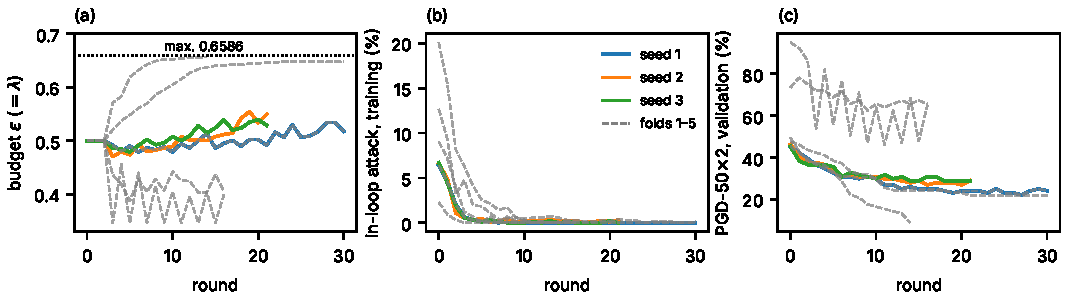
\includegraphics[width=0.92\textwidth]{figs/f_bond_dynamics.pdf}
\caption{Study A on the bond data: game dynamics over rounds (three seeds, solid; five walk-forward folds, dashed grey; round 0 is the undefended forecaster before any update). (a) Budget $\varepsilon{=}\lambda$ set by the controller; dotted, the maximum 0.6586 of Table~\ref{tab:ctrl}. (b) Share of training forecasts broken by the in-loop attack. (c) Share of validation forecasts broken by PGD-50$\times$2, which is never used in training.}
\label{fig:bonddyn}
\end{figure*}

\begin{table}[t]
\centering
\caption{Study A on the bond data: game dynamics (seed 1; \% of forecasts broken, threshold $\tau$). Fresh, stale and strong on validation: PGD-10 against the current forecaster, last round's PGD-10 perturbations replayed, and PGD-50$\times$2. rRMSE: robust validation RMSE, the selection criterion (round 29 selected). Round 0: undefended forecaster.}
\label{tab:bonddyn}
\footnotesize
\setlength{\tabcolsep}{3pt}
\begin{tabular}{rrcccccc}
\toprule
Rd & $s$ & $\varepsilon{=}\lambda$ & Train & Fresh & Stale & Strong & rRMSE\\
\midrule
0 & -- & 0.5000 & 6.4 & 43.3 & -- & 45.2 & --\\
1 & $+0.00$ & 0.5000 & 4.6 & 39.4 & -- & 42.3 & 8.212\\
2 & $+0.00$ & 0.5000 & 2.0 & 36.5 & 38.5 & 39.4 & 8.110\\
3 & $+0.05$ & 0.4919 & 0.6 & 36.5 & 36.5 & 36.5 & 8.030\\
5 & $+0.06$ & 0.4900 & 0.2 & 31.7 & 34.6 & 32.7 & 7.367\\
7 & $+0.08$ & 0.4867 & 0.0 & 30.8 & 29.8 & 30.8 & 7.194\\
10 & $+0.13$ & 0.4788 & 0.0 & 26.9 & 28.8 & 29.8 & 6.854\\
15 & $+0.09$ & 0.4860 & 0.0 & 24.0 & 25.0 & 25.0 & 6.471\\
20 & $-0.01$ & 0.5021 & 0.0 & 24.0 & 23.1 & 24.0 & 6.230\\
25 & $-0.04$ & 0.5068 & 0.0 & 22.1 & 22.1 & 23.1 & 6.136\\
29 & $-0.21$ & 0.5340 & 0.0 & 21.2 & 19.2 & 25.0 & 5.995\\
30 & $-0.11$ & 0.5175 & 0.0 & 20.2 & 21.2 & 24.0 & 6.284\\
\bottomrule
\end{tabular}
\end{table}

\begin{table}[t]
\centering
\caption{Study A on the bond data: loop diagnostics per run. Rounds: rounds run (selected round). Train and strong: share of forecasts broken by the in-loop attack on training data and by PGD-50$\times$2 on validation, at round 0 and in the last round. F$-$S: fresh minus stale response, mean over the second half of the run. Gap: exploitability gap, mean over rounds (points).}
\label{tab:bondruns}
\footnotesize
\setlength{\tabcolsep}{2pt}
\resizebox{\columnwidth}{!}{\begin{tabular}{lcccccc}
\toprule
Run & Rounds & $\varepsilon{=}\lambda$ range & Train (\%) & Strong (\%) & F$-$S & Gap\\
\midrule
Seed 1 & 30 (29) & 0.4785--0.5341 & 6.4$\to$0.0 & 45.2$\to$24.0 & $-0.26$ & 1.73\\
Seed 2 & 21 (15) & 0.4707--0.5544 & 6.6$\to$0.3 & 46.2$\to$28.8 & $-0.67$ & 1.47\\
Seed 3 & 21 (15) & 0.4792--0.5394 & 6.7$\to$0.0 & 45.2$\to$28.8 & $+0.00$ & 1.05\\
Fold 1 & 16 (10) & 0.3877--0.5000 & 9.1$\to$0.0 & 73.4$\to$65.6 & $-0.98$ & 6.05\\
Fold 2 & 30 (27) & 0.5000--0.6485 & 20.1$\to$0.1 & 47.4$\to$21.8 & $-0.17$ & 0.17\\
Fold 3 & 14 (8) & 0.5000--0.6567 & 12.7$\to$0.1 & 49.5$\to$8.8 & $-1.10$ & 1.73\\
Fold 4 & 30 (29) & 0.4785--0.5341 & 6.4$\to$0.0 & 45.2$\to$24.0 & $-0.26$ & 1.73\\
Fold 5 & 16 (10) & 0.3461--0.5000 & 2.3$\to$0.0 & 94.9$\to$65.0 & $-0.53$ & 5.98\\
\bottomrule
\end{tabular}}
\end{table}

In the outcome of the loop (Table~\ref{tab:bondout}), HAD-Stack lowers the worst-case RMSE of the undefended forecaster at both budgets in 8 of 8 seeds and folds, and the paired interval excludes zero in every run (Table~\ref{tab:bondci}). Over the five folds the worst-case RMSE falls from 10.78 to 8.00 at $\varepsilon{=}0.5$ and from 12.81 to 11.41 at $\varepsilon{=}1.0$, and the broken rate from 77.1\% to 56.6\% and from 82.9\% to 72.6\%. On the fixed split the worst-case RMSE falls from 13.14 to 12.06 and from 14.15 to 13.82, and the broken rate from 90.9\% to 89.5\% and from 94.5\% to 92.8\%. The broken rate falls in every run, but its interval excludes zero in only 4 of 8 runs at $\varepsilon{=}0.5$ and 3 of 8 at $\varepsilon{=}1.0$.

\begin{table*}[t]
\centering
\caption{Study A on the bond data: outcome of the loop, HAD-Stack against the undefended forecaster and the fixed-budget forecaster ($\varepsilon{=}0.6586$, $\lambda{=}0.5$), mean $\pm$ std over folds or seeds. Broken: share of test days whose absolute error the worst-case ensemble (Algorithm~\ref{alg:evalR}) raises by more than $\tau$. WC-RMSE: RMSE of each day's largest error over the ensemble. Added: mean increase of the absolute error under the ensemble over its clean value (worst-case MAE minus clean MAE). DA: directional accuracy.}
\label{tab:bondout}
\footnotesize
\setlength{\tabcolsep}{2.2pt}
\resizebox{\textwidth}{!}{\begin{tabular}{lcccccccccc}
\toprule
Model & MAE & RMSE & DA (\%) & Broken 0.5 & Broken 1.0 & WC-RMSE 0.5 & WC-RMSE 1.0 & Added 0.5 & Added 1.0\\
\midrule
\multicolumn{10}{l}{\emph{Five walk-forward folds (131 test days per fold; 122 in fold 5)}}\\
Undefended Two-Head LSTM & 2.825 $\pm$ 1.472 & 4.494 $\pm$ 2.086 & 48.9 $\pm$ 5.1 & 77.1 $\pm$ 12.6 & 82.9 $\pm$ 9.3 & 10.78 $\pm$ 1.49 & 12.81 $\pm$ 1.04 & 6.53 $\pm$ 1.97 & 9.01 $\pm$ 1.93\\
HAD-Stack & 1.770 $\pm$ 1.252 & 2.827 $\pm$ 1.939 & 51.2 $\pm$ 6.2 & 56.6 $\pm$ 30.4 & 72.6 $\pm$ 17.6 & 8.00 $\pm$ 3.41 & 11.41 $\pm$ 2.28 & 4.66 $\pm$ 3.01 & 8.26 $\pm$ 2.74\\
Fixed-budget AT & 0.990 $\pm$ 0.669 & 1.443 $\pm$ 1.152 & 50.3 $\pm$ 6.8 & 45.2 $\pm$ 23.9 & 69.8 $\pm$ 16.0 & 5.71 $\pm$ 2.57 & 10.21 $\pm$ 2.00 & 2.86 $\pm$ 1.73 & 7.59 $\pm$ 2.16\\
\midrule
\multicolumn{10}{l}{\emph{Fixed split, three seeds (254 test days)}}\\
Undefended Two-Head LSTM & 6.055 $\pm$ 0.000 & 8.163 $\pm$ 0.000 & 42.7 $\pm$ 0.0 & 90.9 $\pm$ 0.0 & 94.5 $\pm$ 0.0 & 13.14 $\pm$ 0.00 & 14.15 $\pm$ 0.00 & 6.58 $\pm$ 0.00 & 7.79 $\pm$ 0.01\\
HAD-Stack & 3.877 $\pm$ 0.069 & 6.327 $\pm$ 0.050 & 43.5 $\pm$ 0.0 & 89.5 $\pm$ 1.0 & 92.8 $\pm$ 0.5 & 12.06 $\pm$ 0.13 & 13.82 $\pm$ 0.06 & 7.25 $\pm$ 0.11 & 9.50 $\pm$ 0.04\\
Fixed-budget AT & 2.556 $\pm$ 0.103 & 4.672 $\pm$ 0.137 & 43.7 $\pm$ 0.5 & 79.9 $\pm$ 2.3 & 88.3 $\pm$ 0.5 & 8.30 $\pm$ 0.36 & 12.60 $\pm$ 0.14 & 3.82 $\pm$ 0.35 & 9.16 $\pm$ 0.12\\
\bottomrule
\end{tabular}}
\end{table*}

\begin{table*}[t]
\centering
\caption{Study A on the bond data: HAD-Stack minus the undefended forecaster per run, with paired moving-block bootstrap 95\% intervals. Broken in percentage points; WC-RMSE in the units of the series.}
\label{tab:bondci}
\footnotesize
\setlength{\tabcolsep}{6pt}
\begin{tabular}{lcccc}
\toprule
Run & Broken 0.5 & Broken 1.0 & WC-RMSE 0.5 & WC-RMSE 1.0\\
\midrule
Seed 1 & $-2.8$ $[-6.7,+2.8]$ & $-2.4$ $[-3.5,-0.4]$ & $-1.12$ $[-1.62,-0.70]$ & $-0.40$ $[-0.57,-0.18]$\\
Seed 2 & $-1.2$ $[-3.9,+3.5]$ & $-1.6$ $[-2.8,\phantom{+}0.0]$ & $-1.22$ $[-1.77,-0.75]$ & $-0.35$ $[-0.51,-0.16]$\\
Seed 3 & $-0.4$ $[-2.8,+4.3]$ & $-1.2$ $[-2.0,\phantom{+}0.0]$ & $-0.90$ $[-1.34,-0.51]$ & $-0.24$ $[-0.35,-0.12]$\\
Fold 1 & $-5.3$ $[-13.0,-0.8]$ & $-2.3$ $[-6.9,+0.8]$ & $-0.34$ $[-0.75,-0.07]$ & $-0.20$ $[-0.58,-0.01]$\\
Fold 2 & $-58.8$ $[-75.6,-44.3]$ & $-32.8$ $[-42.0,-19.8]$ & $-6.70$ $[-9.47,-4.63]$ & $-4.26$ $[-5.17,-3.19]$\\
Fold 3 & $-28.2$ $[-45.8,-16.8]$ & $-9.2$ $[-15.3,-3.1]$ & $-3.41$ $[-5.30,-1.78]$ & $-1.80$ $[-2.89,-1.00]$\\
Fold 4 & $-6.9$ $[-12.2,-1.5]$ & $-3.8$ $[-6.9,\phantom{+}0.0]$ & $-1.84$ $[-2.72,-1.16]$ & $-0.59$ $[-0.86,-0.25]$\\
Fold 5 & $-3.3$ $[-9.0,\phantom{+}0.0]$ & $-3.3$ $[-9.0,\phantom{+}0.0]$ & $-1.64$ $[-2.66,-0.69]$ & $-0.19$ $[-0.33,-0.09]$\\
\bottomrule
\end{tabular}
\end{table*}

Unlike on the UPI data, clean accuracy does not deteriorate. Clean RMSE falls in 7 of 8 runs (walk-forward means 4.49 to 2.83, fixed split 8.16 to 6.33) and DA rises from 48.9\% to 51.2\% and from 42.7\% to 43.5\%. A lower worst-case error can therefore come from a better clean fit as well as from a smaller effect of the attack, and the two must be separated. The error the attack adds, the worst-case MAE minus the clean MAE (Table~\ref{tab:bondout}), shrinks under HAD-Stack in folds 2--5 at $\varepsilon{=}0.5$ (walk-forward means 6.53 to 4.66) and in folds 2 and 3 at $\varepsilon{=}1.0$. On the fixed split and in fold 1 it grows (fixed split 6.58 to 7.25 and 7.79 to 9.50), so there the lower worst-case error comes from the better fit alone: on seed 1, white-box PGD-100$\times$5 at $\varepsilon{=}0.5$ raises the RMSE of the undefended forecaster from 8.16 to 13.13 and that of HAD-Stack from 6.29 to 11.98 (Fig.~\ref{fig:bondfc}). Fold 2 shows the opposite case, a robustness gain without a gain in fit: its undefended forecaster is accurate on clean data (RMSE 0.703) yet brittle (65.6\% broken at $\varepsilon{=}0.5$, 6.10 added), and HAD-Stack leaves the clean RMSE nearly unchanged (0.716) while lowering the broken rate to 6.9\% ($-58.8$ points, 95\% CI $[-75.6,-44.3]$) and the added error to 0.38.

The broken rate also depends on the threshold $\tau$ (Fig.~\ref{fig:bondtau}). On seed 1 of the fixed split, HAD-Stack breaks no more test days than the undefended forecaster at $\varepsilon{=}0.5$ for every threshold between $0.25\tau$ and $6\tau$ except $1.125\tau$--$1.25\tau$, but at $\varepsilon{=}1.0$ it breaks more for almost every threshold above $2.1\tau$ (at $4\tau$, 78.3\% against 76.8\%); the fixed-budget forecaster breaks the fewest at $\varepsilon{=}0.5$ for all thresholds, and at $\varepsilon{=}1.0$ the most above $2.9\tau$.

\begin{figure}[t]
\centering
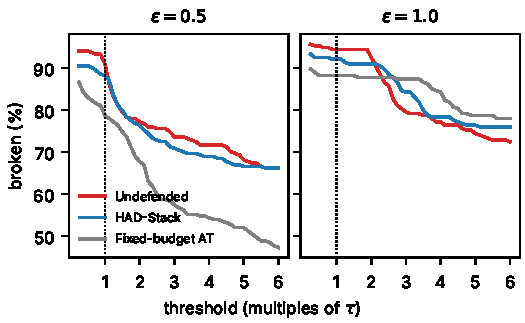
\includegraphics[width=\columnwidth]{figs/f_bond_tau.pdf}
\caption{Study A on the bond data, fixed split, seed 1: broken rate under the worst-case ensemble as a function of the threshold, in multiples of $\tau$ (the training-set standard deviation of the daily change; dotted, the threshold used in the tables).}
\label{fig:bondtau}
\end{figure}

\begin{figure*}[t]
\centering
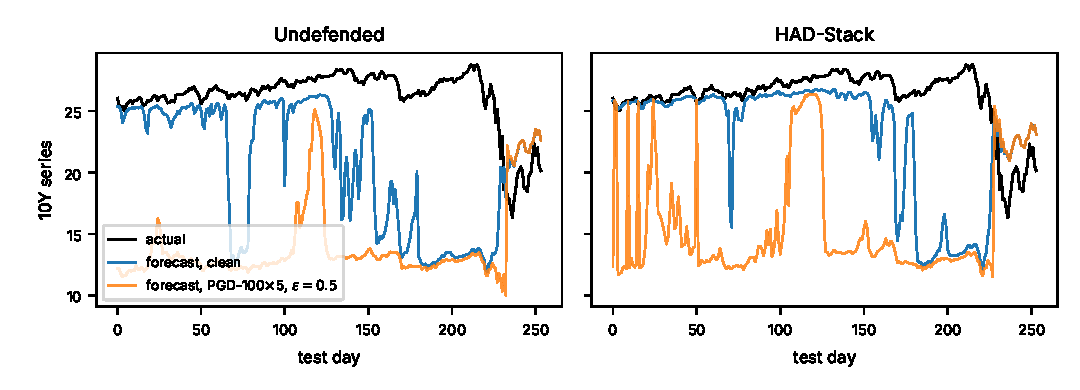
\includegraphics[width=0.8\textwidth]{figs/f_bond_forecast.pdf}
\caption{Study A on the bond data, fixed split, seed 1: the realised 10-year series and the forecasts \eqref{eq:hybrid} on the 254 test days, clean and under white-box PGD-100$\times$5 (squared-error loss) at $\varepsilon{=}0.5$. RMSE clean/attacked: undefended 8.16/13.13, HAD-Stack 6.29/11.98.}
\label{fig:bondfc}
\end{figure*}

The fixed-budget forecaster, trained at the controller's maximum budget throughout, has a lower worst-case RMSE than HAD-Stack at both budgets in all eight runs (walk-forward means 5.71 and 10.21) and a lower clean RMSE (1.44). On these data the controller holds the budget near or below 0.5 in six of the eight runs, so HAD-Stack trains against a weaker attacker than the fixed-budget forecaster does.

\subsection{Computational cost and scaling}\label{sec:cost}
On one CPU thread (Intel Xeon, 2.10 GHz; fixed split, 18,475 training rows), the three Hamiltonian solves of Algorithm~\ref{alg:ctrl} take 41.6 ms per round in the original runs (about 1.2 s over 30 rounds, under 0.1\% of training time; Section~\ref{sec:cpugpu} gives a separate solver benchmark). A HAD-Stack epoch takes 42.7 s, about 4.9 times a clean epoch (8.7 s), because each batch runs the 10-step attack of Algorithm~\ref{alg:pgd}; a full 30-round run takes an estimated 28.5 min. A re-implementation of FraudTransformer (70,593 parameters, as in Section~\ref{sec:detA}) timed on inputs of the data's shape, where the cost of a step does not depend on feature values, gives 7.5 s per clean epoch and 50.0 s per HAD-Stack epoch (means of three epochs). One worst-case white-box evaluation of one model at one budget (682 fraud rows) takes 105 s in the original runs.

Per round, training costs $O\big(n\,(1+n_{\mathrm{PGD}})\,T_{\mathrm{fb}}\big)$ for $n$ transactions, $n_{\mathrm{PGD}}{=}10$ attack steps and $T_{\mathrm{fb}}$ the time of one forward--backward pass, plus an $O(1)$ Hamiltonian solve; inference costs $O(n\,T_{\mathrm{fwd}})$. Measured throughput is constant in $n$ (Table~\ref{tab:scale}): about 2,500 rows/s for clean training up to $10^6$ rows, about 380 rows/s for HAD-Stack training up to $3{\times}10^5$ rows, and about 16,500 rows/s for inference up to $10^6$ rows. At these rates one HAD-Stack epoch over $10^6$ transactions would take about 44 min on one thread, and scoring the 14 billion monthly UPI transactions~\cite{npci2024} (about 5,400 per second on average) would occupy about one third of one such thread; these are projections from measured throughput.

\begin{table}[t]
\centering
\caption{Study A: measured scaling (one thread, Intel Xeon 2.10 GHz; re-implementation on inputs of the data's shape; one run per size)}
\label{tab:scale}
\footnotesize
\begin{tabular}{lrrr}
\toprule
Task & Rows & Time (s) & Rows/s\\
\midrule
Inference & 10,000 & 0.8 & 12,633\\
 & 100,000 & 5.9 & 16,854\\
 & 1,000,000 & 60.8 & 16,458\\
Clean training epoch & 18,475 & 7.7 & 2,410\\
 & 100,000 & 39.0 & 2,567\\
 & 1,000,000 & 397.2 & 2,517\\
HAD-Stack training epoch & 18,475 & 48.6 & 380\\
 & 100,000 & 260.4 & 384\\
 & 300,000 & 806.1 & 372\\
\bottomrule
\end{tabular}
\end{table}

%=====================================================================
\section{Results of Study B}\label{sec:resB}
%=====================================================================
\subsection{Hamiltonian validation and the GNN baseline}
All three systems converge within 50 self-consistent iterations (Table~\ref{tab:sc}), consistent with the convergence analysis of Section~\ref{sec:conv}. The order parameters of $H_1$ and $H_2$ are of order $10^{-6}$ because the implemented iteration evaluates $\langle ab\rangle$ and $\langle ac\rangle$, which vanish in the single-excitation ground state (Section~\ref{sec:h12}); the listed values are therefore residuals of the iteration rather than physical coherences, and their exact size depends on the initial value and stopping tolerance. The effective coupling is set by the drive term, as under the complex treatment of Study~A. The qubit-mapped $H_1$ and $H_2$ match the direct construction exactly.

The residual GNN (Table~\ref{tab:gnn}) reaches near-zero Frobenius loss on $H_1$ ($4.3{\times}10^{-5}$) and $H_2$ ($1.0{\times}10^{-4}$) but degrades on $\HV$ ($2.0{\times}10^{-2}$), and on random Hamiltonians of dimension 32 and 64 the loss reaches 1.62 and 10.3. The GNN predicts $H$ directly; the Q-VAE instead learns a latent encoding of the ground state, which is the object the game attacks.

\begin{table}[t]
\centering
\caption{Study B: self-consistent solutions and qubit-mapping check (Hermitian eigensolver, Section~\ref{sec:spec}; order parameters are iteration residuals, Section~\ref{sec:h12})}
\label{tab:sc}
\footnotesize
\begin{tabular}{lcccc}
\toprule
System & dim & Order param. & $E_0$ & $\|H_{\mathrm{JW}}-H_{\mathrm{dir}}\|_F$\\
\midrule
$H_1$ & 4 & $3.2{\times}10^{-6}$ & $-0.1118$ & 0 (exact)\\
$H_2$ & 4 & $4.9{\times}10^{-6}$ & $-0.0500$ & 0 (exact)\\
$\HV$ & 16 & $\approx0$ & $-2.0004$ & N/A (Pauli)\\
\bottomrule
\end{tabular}
\end{table}

\begin{table}[t]
\centering
\caption{Study B: residual GNN Hamiltonian prediction and dimension scaling}
\label{tab:gnn}
\footnotesize
\setlength{\tabcolsep}{4pt}
\begin{tabular}{lccccc}
\toprule
System & dim & Params & Mem & Loss & s/ep\\
\midrule
$H_1$ & 4 & 21K & 0.08 MB & $4.3{\times}10^{-5}$ & 0.002\\
$H_2$ & 4 & 21K & 0.08 MB & $1.0{\times}10^{-4}$ & 0.002\\
$\HV$ & 16 & 29K & 0.12 MB & $2.0{\times}10^{-2}$ & 0.002\\
\midrule
\multicolumn{6}{l}{\emph{Random Hamiltonians}}\\
-- & 32 & 147K & 0.59 MB & 1.62 & 0.003\\
-- & 64 & 844K & 3.38 MB & 10.3 & 0.004\\
\bottomrule
\end{tabular}
\end{table}

\subsection{Classical check on MNIST}
The Stackelberg + QPSO loop is first checked on MNIST (Fig.~\ref{fig:mnist}): after 20 epochs the defender reaches 99.38\% clean accuracy and 93.37\% PGD-20 robust accuracy at $\varepsilon{=}0.15$, with PSNR above 49 dB, and the leader's attack success falls from 13.1\% (epoch 1) to 6.1\% (epoch 20). This is diagnostic (a) of Definition~\ref{def:diag}: the follower adapts to the leader. It does not by itself establish convergence to an equilibrium.

\begin{figure}[t]
\centering
\includegraphics[width=\columnwidth]{figs/q_mnist.pdf}
\caption{Study B, classical check on MNIST. (a) Clean and PGD-20 robust accuracy over training. (b) Leader attack success per epoch.}
\label{fig:mnist}
\end{figure}

\subsection{The quantum game}
Table~\ref{tab:qgame} answers Q3. On the two 4-dimensional systems the defender dominates: robustness ratios are 6.61 ($H_1$) and 5.70 ($H_2$) and the leader's energy gain is negative ($-0.015$, $-0.019$). On the 16-dimensional $\HV$ the attacker gains the advantage (ratio 0.48), although $\Delta E$ is again negative ($-0.017$). QPSO supplied the leader's move in most epochs (30, 26 and 28 of 30). Fig.~\ref{fig:advex} shows representative clean and adversarial reconstructions; the fidelity between them is 0.454, 0.324 and 0.118 for $H_1$, $H_2$ and $\HV$, and the perturbations remain structured and localised.

\begin{table}[t]
\centering
\caption{Study B: quantum Stackelberg game (30 epochs, $\varepsilon{=}0.1$). ALS/QPSO: epochs in which each search supplied the leader's move.}
\label{tab:qgame}
\footnotesize
\begin{tabular}{lcccccc}
\toprule
System & $\cL_c$ & $\cL_a$ & Rob. & $\Delta E$ & ALS & QPSO\\
\midrule
$H_1$ & 0.884 & 0.134 & 6.61 & $-0.015$ & 0 & 30\\
$H_2$ & 1.263 & 0.222 & 5.70 & $-0.019$ & 4 & 26\\
$\HV$ & 0.245 & 0.514 & 0.48 & $-0.017$ & 2 & 28\\
\bottomrule
\end{tabular}
\end{table}

\begin{figure}[t]
\centering
\includegraphics[width=\columnwidth]{figs/q_advex.pdf}
\caption{Study B adversarial examples. Top: clean (blue) and adversarially perturbed (red) state amplitudes for $H_1$, $H_2$ and $\HV$. Bottom: perturbation magnitude per amplitude, with the fidelity between clean and adversarial reconstructions. The panels label $\HV$ as $H_3$.}
\label{fig:advex}
\end{figure}

\subsection{Convergence of the loop}
The rolling standard deviation of $\Delta E$ (Fig.~\ref{fig:conv}) falls below 0.01 by epoch 6 for $H_1$ and $H_2$, indicating that the loop becomes stationary; for $\HV$ it remains at 0.088 after 30 epochs, so the game has not stabilised. This matches the dimension dependence of Table~\ref{tab:qgame}: the larger latent space of $\HV$ ($q{=}4$) admits more complex dynamics that need more epochs or stronger optimisation.

\begin{figure*}[t]
\centering
\includegraphics[width=0.85\textwidth]{figs/q_conv.pdf}
\caption{Study B convergence: leader energy gain $\Delta E$ (solid) and its rolling standard deviation, reported as ``Nash gap'' (dashed), for $H_1$ ($d{=}4$), $H_2$ ($d{=}4$) and $\HV$ ($d{=}16$; labelled $H_3$ in the panels).}
\label{fig:conv}
\end{figure*}

\subsection{Ablations}
Table~\ref{tab:qabl} reports ablations on $H_1$ (15 epochs, $\varepsilon{=}0.1$). Without an attack the ratio is 1.0. Among the attacker variants (rows 2--4), ALS alone succeeds in 6.7\% of attempts with the lowest fidelity (0.19), QPSO alone in 53.3\% (fidelity 0.38), and the combined ALS+QPSO leader in 60.0\%, the highest attack success; the defender trained against it attains the highest fidelity of the three (0.59). The very high ratios of rows 2, 3 and 5 arise from adversarial losses of 0.02--0.04 and should not be read as stronger defences. Replacing parameter-shift gradients by finite differences lets the attack succeed in 100\% of attempts and lowers fidelity from 0.59 to 0.46; replacing FC-VQC by a plain VQC gives a ratio of 2.35 (fidelity and attack success not recorded); and a simultaneous min--max game gives a ratio of 3.28 compared with 2.47 for the sequential game (attack success was not recorded for these two rows).

\begin{table}[t]
\centering
\caption{Study B: ablations on $H_1$ ($q{=}2$, dim 4, 15 epochs, $\varepsilon{=}0.1$)}
\label{tab:qabl}
\footnotesize
\setlength{\tabcolsep}{3pt}
\begin{tabular}{rlcccccc}
\toprule
\# & Method & $\cL_c$ & $\cL_a$ & Rob. & $\Delta E$ & Fid. & Atk.\ (\%)\\
\midrule
1 & No attack & 0.37 & 0.37 & 1.00 & 0.00 & 1.00 & 0.0\\
2 & ALS only & 0.49 & 0.03 & 16.0 & $-0.03$ & 0.19 & 6.7\\
3 & QPSO only & 0.76 & 0.04 & 17.3 & $+0.00$ & 0.38 & 53.3\\
4 & ALS+QPSO & 1.50 & 0.61 & 2.47 & $-0.00$ & 0.59 & 60.0\\
\midrule
5 & Finite-difference & 0.31 & 0.02 & 17.2 & $+0.00$ & 0.46 & 100\\
6 & Plain VQC & 0.31 & 0.13 & 2.35 & $-0.05$ & -- & --\\
7 & Min--max game & 0.52 & 0.16 & 3.28 & $-0.05$ & -- & --\\
\bottomrule
\end{tabular}
\end{table}

\subsection{Latent-space robustness}\label{sec:latrob}
Under the same ALS+QPSO attack at $\varepsilon{=}0.1$ on $H_1$, the adversarially trained Q-VAE reaches a reconstruction fidelity of 0.658 against 0.174 for a standard Q-VAE, a factor of 3.78 (Fig.~\ref{fig:fid}); the adversarial model is higher at every tested budget in $[0.02,0.3]$. Its decoder has a larger Jacobian norm (9.22 vs.\ 2.29), so robustness is not obtained by flattening the decoder globally: a small Lipschitz constant $L_\psi$ is sufficient for a small payoff by Theorem~\ref{thm:energy}, but it is not what the Stackelberg-trained decoder uses.

\begin{figure}[t]
\centering
\includegraphics[width=0.92\columnwidth]{figs/q_fid.pdf}
\caption{Study B: reconstruction fidelity on $H_1$ under the ALS+QPSO attack as a function of $\varepsilon$, for the standard and the Stackelberg-trained Q-VAE.}
\label{fig:fid}
\end{figure}

\subsection{Computational structure}\label{sec:qstruct}
Both inner computations are parallel. All timings in this subsection were measured on an AMD Ryzen 9 CPU (Section~\ref{sec:qc}). The $2P$ shifted circuits of \eqref{eq:ps} are independent, so with $n_{\mathrm w}$ workers $T^{\mathrm{par}}_{\mathrm{PS}}=\lceil 2P/n_{\mathrm w}\rceil T_{\mathrm{eval}}$ and the ideal speedup is $n_{\mathrm w}$; QPSO needs $N_pN_{\mathrm{it}}$ independent fitness evaluations per search ($N_{\mathrm{it}}$ iterations), $O(N_pN_{\mathrm{it}}\,T_{\mathrm{eval}}/n_{\mathrm w})$ in parallel. With four workers the measured parameter-shift speedup is below 1 for $q\le5$ (0.56--0.81) because of scheduling overhead and reaches 1.21 at $q{=}6$ (per-block $P=3qK$ from 12 to 36). QPSO throughput rises from $2.3{\times}10^5$ to $4.8{\times}10^6$ evaluations per second as the swarm grows from 10 to 320 particles. State-vector simulation costs $O(BKq\,2^q)$ per FC-VQC forward pass, $O(P\,2^q)$ per parameter-shift gradient, $O(d\,2^q)$ per ALS sweep and $O(N_p2^q)$ per QPSO iteration. Over the components of Table~\ref{tab:runtime}, parameter-shift evaluation takes 64--67\% of the summed time, making it the main target for GPU batching or scheduling across multiple quantum processing units (QPUs). A full game step grows from 0.75 s at $q{=}2$ to 52.88 s at $q{=}5$ (Table~\ref{tab:runtime}).

\begin{table}[t]
\centering
\caption{Study B: component runtime per step and end-to-end game step (seconds; AMD Ryzen 9 CPU)}
\label{tab:runtime}
\footnotesize
\setlength{\tabcolsep}{3pt}
\begin{tabular}{ccccccc}
\toprule
$q$ & FC-VQC & Param-shift & QPSO & Q-VAE & Full step & 5 epochs\\
\midrule
2 & 0.001 & 0.007 & $<$0.001 & 0.003 & 0.75 $\pm$ 0.00 & 3.8\\
3 & 0.004 & 0.018 & $<$0.001 & 0.006 & 4.36 $\pm$ 0.01 & 21.8\\
4 & 0.007 & 0.043 & $<$0.001 & 0.014 & 16.07 $\pm$ 0.04 & 80.4\\
5 & 0.017 & 0.100 & $<$0.001 & 0.034 & 52.88 $\pm$ 0.14 & 264.4\\
6 & 0.059 & 0.319 & $<$0.001 & 0.107 & -- & --\\
\bottomrule
\end{tabular}
\end{table}

%=====================================================================
\section{Discussion}\label{sec:disc}
%=====================================================================
\textbf{Q1: the loop functions as a game in both studies.} In Study~A every diagnostic of Definition~\ref{def:diag} behaves as a two-player loop should: the follower's payoff falls from 26.5\% to 3.3\% while the leader's budget rises, fresh responses differ from stale ones while the defender is changing and coincide once it is stationary, and a stronger attack that is never used in training also succeeds less often. The outcome of the loop is a detector that keeps 70.3\% and 53.0\% of fraud detected under worst-case attack, against 51.6\% and 18.1\% undefended. On a second, public card-fraud dataset, with unchanged hyperparameters, the same diagnostics hold and HAD-Stack keeps 67.7\% and 48.6\% against 52.0\% and 32.5\%, above the undefended detector at both budgets in 8 of 8 runs (Section~\ref{sec:verA}). The same loop, with the controller and its hyperparameters unchanged, also works on a regression model: on the bond data the in-loop attack's success falls to 0.0--0.3\% in every run, PGD-50$\times$2 falls in all eight, fresh and stale responses agree to within one validation window over the second halves of the runs, and the forecaster's worst-case RMSE falls at both budgets in 8 of 8 runs (Section~\ref{sec:resR}). The outcome is weaker than on the fraud data: the error the attack adds shrinks only in four of eight runs at $\varepsilon{=}0.5$ and two at $\varepsilon{=}1.0$, so on the fixed split the gain comes from a better clean fit. In Study~B the leader's success falls over training on MNIST (13.1\% to 6.1\%), and the energy-gain trajectories of the 4-dimensional systems become stationary within 6 epochs. In both studies the stationary point is an approximate one: Study~A's exploitability gap stays near 12 points on the UPI data; on the card data it is about 1 point, yet the worst-case ensemble still breaks 13.9\% and 38.4\% of detected fraud; and Study~B's $\HV$ game has not stabilised after 30 epochs. Neither loop differentiates through the follower's best response (Remark~\ref{rem:labels}), so neither is guaranteed to reach the Stackelberg equilibrium \eqref{eq:se}.

\textbf{Q2: the Hamiltonian solutions are well defined.} For $H_1$ and $H_2$ this is proved: their spectrum is explicit (Theorem~\ref{thm:spec}) and their iterations contract by exactly 0.7 per step to $\Delta_j=0$ (Theorem~\ref{thm:sc}). For $\HV$, Theorem~\ref{thm:sc} reduces convergence to the slope of one expectation value, which we measure. Empirically, the self-consistent iterations of all three operators converge geometrically: the $\HV$ field contracts by a factor of 0.5 per iteration and reaches the same fixed point from initial values spanning four orders of magnitude, under both spectral treatments and at every coupling scale the controller visits (Table~\ref{tab:conv}); the two-mode order parameters contract by 0.7 per iteration (Section~\ref{sec:conv}). As a \emph{controller}, the Hamiltonian channel works as specified: the budget is strictly monotone and Lipschitz in the feedback signal (Corollary~\ref{cor:ctrl}) and moves along Table~\ref{tab:ctrl} in the direction that strengthens the attacker as the defender hardens. On the bond data it also lowers the budget when the defender does not harden (folds 1 and 5), and there the signal alternates in sign, so the feedback law \eqref{eq:feedback} can oscillate instead of settling. As a \emph{payoff}, the Hamiltonian gives the game a physically defined objective, the energy shift of the reconstructed state, so that robustness is measured in the quantity the model is meant to preserve, and that quantity is bounded by the fidelity of the reconstruction (Theorem~\ref{thm:energy}); in Study~B that energy is the one of the Hermitian surrogates (Table~\ref{tab:hamcheck}). The solves are cheap: under 0.1\% of Study~A's training time, and batched over 1,000 coupling values 12.5 times faster than one at a time on a CPU (Table~\ref{tab:solvetime}).

\textbf{From classification to regression.} Moving Study~A from fraud detection to bond-yield forecasting changed three task-specific elements and nothing else: the attacker's loss (cross-entropy on the true label becomes the squared forecast error), the coordinates it may change (the features of fraud rows become the market features of a look-back window), and the notion of a broken case (a flipped decision becomes an error increase above $\tau$). The Hamiltonian layer, the control and feedback laws, the reference budget, the optimiser and the checkpoint rule were reused as they are. The diagnostics of Definition~\ref{def:diag} carried over without change, and so did their reading: on all three datasets the follower's in-loop success falls as the leader adapts, and its fresh and stale responses agree once the leader stops changing. What changed is the behaviour of the controller and of the outcome. The budget saturated at its maximum on the UPI data but moved in both directions on the card and bond data, and on two bond folds it alternated; and while robustness cost clean detection on the UPI data, on the card and bond data clean performance did not deteriorate (Sections~\ref{sec:verA} and~\ref{sec:resR}). Because a regression output has no decision threshold, the broken rate depends on $\tau$, and on the fixed split its ranking reverses at large thresholds and $\varepsilon{=}1.0$ (Fig.~\ref{fig:bondtau}). The worst-case RMSE does not depend on $\tau$ and improves in every run, but it mixes fit and robustness; the error the attack adds isolates robustness, and by that measure HAD-Stack helps in half of the runs at $\varepsilon{=}0.5$. A regression study therefore needs both a threshold-free measure and a fit-free one.

\textbf{Q3: dimension shifts the balance.} The defender wins on both 4-dimensional systems and loses on the 16-dimensional one, whose game also fails to become stationary. With only two dimensions tested, this is a change between $d{=}4$ and $d{=}16$, not an established phase transition.

A lesson common to both studies is that the evaluation decides the claim. In Study~A, a 10-step attack overstated robustness about tenfold; restarts, longer attacks, larger budgets and transfer attacks exposed gradient masking. Further pitfalls changed results during this work: an attack that ascended the loss toward the legitimate label made detectors appear to improve under attack; \texttt{eigh} applied to non-Hermitian matrices returned eigenvalues of a different matrix without warning; feature weights applied after projection pushed $\|\delta\|_\infty$ to $2.65\varepsilon$; zero step weights silently exempted 9 of the 18 features from an earlier evaluation attack; selecting the best epoch on the fold being reported inflated cross-validation scores; and removing features with near-perfect single-feature AUC did not remove support leakage. Study~B is evaluated with its own ALS+QPSO leader; an independent, stronger latent-space attack would be the analogue of Study~A's ensemble.

\textbf{Limitations.}
\emph{Scope:} the evaluation asks whether the game loop works and what it produces relative to the undefended model; it does not compare the Hamiltonian controller with other adversarial-training schedules, except the fixed-budget forecaster of the regression study, which is more robust than HAD-Stack (Section~\ref{sec:resR}). \emph{Operators:} the solver iterates $\langle ab\rangle$ and $\langle ac\rangle$ rather than the transition fields \eqref{eq:Delta1}--\eqref{eq:Delta2}, so $\Delta_j=0$ at convergence, and $\HV$ omits the magnetic terms of \eqref{eq:Hfermi} (Sections~\ref{sec:h12} and~\ref{sec:hv}). \emph{Theory:} the Hamiltonian-to-hyperparameter mappings are design choices; Theorems~\ref{thm:spec}--\ref{thm:sc} and Corollary~\ref{cor:ctrl} establish their monotonicity and the convergence of the $H_1$ and $H_2$ iterations, but the contraction of the $\HV$ iteration rests on a measured slope, Theorem~\ref{thm:energy} assumes a Lipschitz constant $L_\psi$ that we do not estimate, the loop itself is not proved to converge (Remark~\ref{rem:labels}), and the continuous-time model \eqref{eq:diffgame} motivates the loop but is not analysed. \emph{Controller:} $H_1$ and $H_2$ share their spectra at the base parameters, so $\lambda$ is tied to $\varepsilon$; on the UPI data the controller reached its maximum budget at round 7 and stayed there, and on the bond data it oscillated in two of eight runs; the $\HV$ field is unused in the control law; the curriculum direction and weight floor were chosen after observing an earlier variant, and all reported runs use new seeds and folds. \emph{Data:} Study~A's main experiments use one synthetic, nearly separable dataset whose relation to real UPI fraud is not validated; the verification on real card transactions (Section~\ref{sec:verA}) uses anonymised principal-component features and has 74--99 fraud cases per test set; training and inference scale linearly up to $10^6$ rows (Section~\ref{sec:cost}), but production serving~\cite{amodei2016} was not tested. The regression study uses one released forecaster on one series of 1,318 days; on these data its clean error exceeds that of a no-change forecast (fixed split: MAE 6.06 against 0.30), so much of HAD-Stack's gain there reflects a better fit: on the fixed split and in fold 1 the attack adds more error to HAD-Stack's forecasts than to the undefended ones, and the threshold sensitivity of Fig.~\ref{fig:bondtau} was computed for one seed. Study~B uses noiseless state-vector simulation and small systems (dimension at most 16), reports single runs, and learns ground states of the Hermitian surrogates of the shared operators (Table~\ref{tab:hamcheck}). GPU timings of the Hamiltonian solver were not measured.

%=====================================================================
\section{Conclusion}
%=====================================================================
We formulated adversarial learning as a Hamiltonian--Stackelberg game---players, strategies, payoffs, best responses, Stackelberg equilibrium, a round-indexed loop with a differential-game limit, a Hamiltonian channel and loop diagnostics---and instantiated it with one family of non-Hermitian open-system operators, with identical parameters, in two settings: through its complex spectrum and through Hermitian-solver ground states. The self-consistent iterations that define these operators converge geometrically to fixed points independent of their starting values, provably so for the two-mode operators, whose spectrum we give in closed form, and a batched solver computes them on CPU or GPU. The closed form makes the controller's budget strictly monotone and Lipschitz in its feedback signal, and the energy payoff is bounded by the fidelity of the reconstruction. As a controller of a fraud detector's adversarial training, the Hamiltonian channel drives a working attacker--defender loop: the attacker's in-loop success falls as its budget grows, the follower's response becomes stationary, and the trained detector keeps 70.3\% and 53.0\% of fraud detected under worst-case attack at $\varepsilon{=}0.5$ and $1.0$, against 51.6\% and 18.1\% undefended; on a second, public card-fraud dataset, with unchanged hyperparameters, it keeps 67.7\% and 48.6\% against 52.0\% and 32.5\%. Applied without change to regression, to a Two-Head LSTM that forecasts the 10-year Indian government bond yield, the same loop lowers the forecaster's worst-case RMSE at both budgets in all eight seeds and folds, partly through a better clean fit; the error the attack adds shrinks in four of eight runs, and fixed-budget training at the controller's maximum is more robust still. As the payoff of a latent-space game on a quantum variational autoencoder, it defines an energy-shift objective under which the defender dominates on 4-dimensional systems and the attacker on a 16-dimensional one, and Stackelberg training raises fidelity under attack from 0.174 to 0.658. Every algorithm is given as pseudocode, so the loop can be reproduced step by step.

\appendices
\section{Pauli expansion of \texorpdfstring{$\HV$}{HV}}\label{app:hv}
With $\HV$ as in \eqref{eq:HV} and $H_{\mathrm{coupling}}(\phi)=\tfrac{i g_1h\phi}{4}(C\,\cE_1+C'\,\cE_1^{*})$, the four Pauli sums are listed below ($\sigma^{\alpha}_{k}$ acts on qubit $k$; products are tensor products; $I$ is the $16{\times}16$ identity). They are generated from the reference solver; rebuilding $\HV$ from this listing reproduces the solver matrix to $10^{-12}$.
{\footnotesize
\par\noindent $C={}$$\sigma_{0}^{x}\,-\,i\sigma_{0}^{y}\,-\,\sigma_{2}^{y}\,+\,i\sigma_{2}^{x}\,+\,i\sigma_{1}^{z}\,\sigma_{0}^{y}\,-\,\sigma_{1}^{z}\,\sigma_{0}^{x}\,-\,i\sigma_{3}^{z}\,\sigma_{2}^{x}\,\sigma_{1}^{z}\,+\,\sigma_{3}^{z}\,\sigma_{2}^{y}\,\sigma_{1}^{z}$.

\par\noindent $C'={}$$\sigma_{2}^{x}\,-\,i\sigma_{2}^{y}\,+\,i\sigma_{0}^{x}\,-\,\sigma_{0}^{y}\,-\,\sigma_{1}^{y}\,\sigma_{0}^{x}\,-\,i\sigma_{1}^{y}\,\sigma_{0}^{y}\,+\,i\sigma_{3}^{y}\,\sigma_{2}^{y}\,\sigma_{1}^{x}\,-\,\sigma_{3}^{z}\,\sigma_{2}^{y}\,\sigma_{1}^{x}$.

\par\noindent $D_\eta={}$$(4\,-\,8i)I\,+\,5\sigma_{0}^{z}\,-\,4(1\,+\,1i)\sigma_{1}^{z}\,+\,4i\sigma_{1}^{x}\,+\,3\sigma_{1}^{y}\,+\,4i\sigma_{2}^{z}\,-\,(5\,+\,3i)\sigma_{1}^{z}\,\sigma_{0}^{z}\,+\,\sigma_{1}^{z}\,\sigma_{0}^{z}\,-\,3i\sigma_{1}^{x}\,\sigma_{0}^{z}\,+\,2i\sigma_{2}^{z}\,\sigma_{0}^{z}\,+\,2i\sigma_{2}^{y}\,\sigma_{0}^{y}\,+\,4i\sigma_{3}^{z}\,\sigma_{1}^{z}\,-\,\sigma_{2}^{y}\,\sigma_{1}^{y}\,\sigma_{0}^{x}\,-\,i\sigma_{2}^{y}\,\sigma_{1}^{y}\,\sigma_{0}^{y}\,+\,i\sigma_{2}^{y}\,\sigma_{1}^{y}\,\sigma_{0}^{z}\,-\,\sigma_{2}^{y}\,\sigma_{1}^{x}\,\sigma_{0}^{y}\,-\,i\sigma_{2}^{y}\,\sigma_{1}^{z}\,\sigma_{0}^{x}\,-\,i\sigma_{2}^{x}\,\sigma_{1}^{z}\,\sigma_{0}^{y}\,+\,\sigma_{2}^{x}\,\sigma_{1}^{z}\,\sigma_{0}^{x}\,-\,\sigma_{2}^{x}\,\sigma_{1}^{y}\,\sigma_{0}^{y}\,+\,\sigma_{3}^{z}\,\sigma_{2}^{y}\,\sigma_{0}^{y}\,-\,\sigma_{3}^{z}\,\sigma_{2}^{x}\,\sigma_{0}^{x}\,+\,i\sigma_{3}^{z}\,\sigma_{2}^{z}\,\sigma_{0}^{y}\,-\,\sigma_{3}^{z}\,\sigma_{3}^{x}\,\sigma_{0}^{x}\,-\,2i\sigma_{3}^{z}\,\sigma_{2}^{y}\,\sigma_{0}^{x}\,-\,i\sigma_{3}^{z}\,\sigma_{2}^{x}\,\sigma_{0}^{y}\,-\,4i\sigma_{3}^{z}\,\sigma_{2}^{y}\,\sigma_{1}^{z}\,+\,(1\,-\,3i)\sigma_{3}^{z}\,\sigma_{2}^{y}\,\sigma_{1}^{z}\,\sigma_{0}^{x}\,-\,i\sigma_{3}^{z}\,\sigma_{2}^{y}\,\sigma_{1}^{x}\,\sigma_{0}^{x}\,+\,\sigma_{3}^{z}\,\sigma_{2}^{y}\,\sigma_{1}^{x}\,\sigma_{0}^{y}\,+\,\sigma_{3}^{z}\,\sigma_{2}^{x}\,\sigma_{1}^{z}\,\sigma_{0}^{x}\,-\,i\sigma_{3}^{z}\,\sigma_{2}^{x}\,\sigma_{1}^{z}\,\sigma_{0}^{y}$.

\par\noindent $D_0={}$$(4\,-\,2i)I\,+\,(4\,+\,2i)\sigma_{0}^{z}\,-\,(4\,-\,2i)\sigma_{1}^{z}\,+\,2i\sigma_{1}^{x}\,+\,\sigma_{1}^{y}\,-\,(5\,+\,1i)\sigma_{1}^{z}\,\sigma_{0}^{z}\,-\,2i\sigma_{1}^{x}\,\sigma_{0}^{z}\,-\,\sigma_{1}^{y}\,\sigma_{0}^{z}\,-\,2\sigma_{2}^{y}\,\sigma_{0}^{y}\,+\,2\sigma_{2}^{x}\,\sigma_{0}^{x}\,-\,\sigma_{2}^{y}\,\sigma_{1}^{y}\,\sigma_{0}^{x}\,-\,i\sigma_{2}^{y}\,\sigma_{1}^{y}\,\sigma_{0}^{y}\,+\,i\sigma_{2}^{y}\,\sigma_{1}^{x}\,\sigma_{0}^{x}\,-\,\sigma_{2}^{x}\,\sigma_{1}^{y}\,\sigma_{0}^{y}\,+\,\sigma_{2}^{y}\,\sigma_{1}^{z}\,\sigma_{0}^{x}\,+\,i\sigma_{2}^{y}\,\sigma_{1}^{z}\,\sigma_{0}^{x}\,+\,\sigma_{2}^{x}\,\sigma_{1}^{z}\,\sigma_{0}^{y}\,-\,\sigma_{2}^{x}\,\sigma_{1}^{z}\,\sigma_{0}^{x}\,-\,\sigma_{3}^{z}\,\sigma_{2}^{y}\,\sigma_{0}^{y}\,-\,i\sigma_{3}^{z}\,\sigma_{2}^{y}\,\sigma_{0}^{x}\,-\,i\sigma_{3}^{z}\,\sigma_{2}^{x}\,\sigma_{0}^{y}\,+\,\sigma_{3}^{z}\,\sigma_{2}^{x}\,\sigma_{0}^{x}\,-\,2\sigma_{3}^{z}\,\sigma_{2}^{x}\,\sigma_{1}^{z}\,\sigma_{0}^{x}\,-\,\sigma_{3}^{z}\,\sigma_{2}^{y}\,\sigma_{1}^{x}\,\sigma_{0}^{x}\,-\,i\sigma_{3}^{z}\,\sigma_{2}^{x}\,\sigma_{1}^{x}\,\sigma_{0}^{y}\,+\,(1\,-\,1i)\sigma_{3}^{z}\,\sigma_{2}^{y}\,\sigma_{1}^{z}\,\sigma_{0}^{x}\,+\,2\sigma_{3}^{z}\,\sigma_{2}^{y}\,\sigma_{1}^{z}\,\sigma_{0}^{y}\,-\,i\sigma_{3}^{z}\,\sigma_{2}^{y}\,\sigma_{1}^{x}\,\sigma_{0}^{x}\,+\,\sigma_{3}^{z}\,\sigma_{2}^{y}\,\sigma_{1}^{x}\,\sigma_{0}^{y}$.

}

\section*{Acknowledgement}
Authors are listed in random order; the order does not reflect relative contributions.

\bibliographystyle{IEEEtran}
\bibliography{refs}

\end{document}
